\chapter{Probabilistic Modelling}
\label{c:ml-background}

% \textbf{Summary.} In this chapter, we provide a brief background on probabilistic mixture models. Both finite and infinite mixture models are used in Chapters~\ref{c:matching} and \ref{c:precursor-clustering} for the grouping of related peaks in the same LC-MS run. Next, we introduce a hierarchical mixture models that allows for the grouping of peaks across multiple runs. This is used in Chapter~\ref{c:hdp}. Finally we introduce topic modelling in the form of Latent Dirichlet Allocation. This is used in Chapter~\ref{c:lda} to infer the presence of related peaks that potentially correspond to substructures shared by metabolites.

\section{Introduction}

As described in Chapter~\ref{c:background}, the raw data produced from liquid chromatography mass spectrometry (LC-MS) measurements has to be processed through a data pre-processing pipeline before further analysis. From the peak detection step, we obtain points on the ion chromatograms having mass-to-charge (m/z), retention time (RT) and intensity values. We call each point a \emph{peak}. The nature of LC-MS measurements means that a compound being analysed generates multiple peaks. At the heart of this thesis is the grouping of these peaks that are structurally or chemically related, and using the grouping to improve other steps (such as the alignment and identification steps) in the pipeline. The problem of finding these groups of related peaks can be approached as an unsupervised learning problem. In the unsupervised learning approach, broadly speaking our task is to separate peaks into \emph{clusters}, where members of the cluster are related through sharing some commonalities, e.g. from being the ionisation products of the same compound or from sharing chemical substructures.

Numerous methods exist to perform data clustering in an unsupervised manner \cite{xu2005survey, Jain2010}. In probabilistic modelling, one way to do this is to try and explain the generative process that produces the observed data. This results in a generative model. Peaks generated from the same underlying cause in the model can then be assigned to the same cluster. Modelling the data in this manner has some advantages in comparison to other distance-based clustering methods, such as e.g. hierarchical clustering that has also been applied to peak data \cite{DeSouza2006, Frank2007}. A generative model provides more than just clustering. It is often easier to extract from a generative model a hint as to \emph{why} the observed data points are clustered, and this insight can be very useful in certain applications. Additionally, through specifying the appropriate likelihood functions, generative modelling also provides a flexible way of specifying how data points should be clustered, while prior assumptions can be incorporated into the model in a principled manner.

Generative modelling has been applied to LC-MS data. In \cite{Rogers2012}, mixture model clustering is used to cluster LC-MS peaks in the same run by their chromatographic profiles. Mixture models are the building blocks of more complex generative models. In mixture models, it is assumed that the observed data can be explained by the presence of some latent variables. These variables are `latent' as they are not directly observed, rather their presence is inferred from the observed data. The assumption made in \cite{Rogers2012} is that ionisation product peaks that are related share similar chromatographic profiles. Given $N$ peaks in the data, the method computes the pairwise Pearson correlation values for the chromatographic profiles of all peaks, resulting in an $N$-by-$N$ matrix of Pearson correlation values. The likelihood of an entry in this matrix is described by a mixture of two components: an exponential-type distribution to describe the correlation values of peaks in the same cluster and a Gaussian distribution to describe the correlation values of peaks in different clusters. 

Along a similar line, mixture model clustering is also used in MetAssign \cite{Daly2014} to perform the probabilistic annotations of ionisation product types and formulae to peak data. It is assumed in MetAssign that a prior knowledge of the form of known formulae is provided. Theoretical peaks are then generated using the provided formulae. The likelihood of an observed peak is computed based on how well the observed m/z, RT and intensity values fit the theoretical peaks. Other applications of probabilistic modelling on mass spectrometry data include modelling the assignment of formulae to peaks \cite{Rogers2009a, Silva2014}, modelling the fragmentation events of tandem mass spectrometry data, where the separation is performed using liquid chromatography (CMF-ESI, \cite{Allen2014}) or gas chromatography (CFM-EI, \cite{Allen2016}). Machine learning techniques in general have also been applied to mass spectrometry data, e.g. for the predictions of retention time \cite{Creek2011, Cao2015, Stanstrup2015} and the characteristic fingerprints of compounds from fragmentation data \cite{Heinonen2012a, Duhrkop2015}. 

% A general survey of computational problems in the processing of mass spectrometry data can be found in \cite{Smith2014}.

% The pre-processing of LC-MS data in a pipeline involves many sequential steps. At each step, often the `true answer' (the ground truth) as to the correctness of the step is unknown or known only for a small number of peaks. In particular for the peak grouping step, this means that in many cases, we do not know for certain what the true grouping is. 

\section{Mixture Model Clustering}
\label{sub:background-mixture-model-clustering}

As an example of the thinking process behind generative modelling, we see that during liquid chromatography, metabolites are separated by their chemical properties. From mass spectrometry, ionisation product peaks are produced from the same metabolites. These peaks will co-elute and have similar chromatographic profiles, including broadly similar RT values. A group of observed peaks having similar retention time (RT) values can be therefore be modelled as being generated by the same metabolite, and in this case, although the metabolite is not directly observed, its presence can be inferred based on the observed data. Peaks that are related to the same compound can therefore be clustered according to their RT values. Let our LC-MS run be represented as $\mathbf{y}=\{y_{1},y_{2},...,y_{n}\}$ where each $y_n$ is the RT value of a peak. 

A principled way to model a generative process is through Bayesian inference. Suppose $\theta$ is the parameter of interest to the generative process that produces the data $\mathbf{y}$. In Bayesian inference, we begin by specifying a prior distribution over the model parameter $\theta$. Through the application of Bayes rule, this prior distribution is updated by the likelihood of seeing the observed data given our prior hypothesis on $\theta$, resulting in a posterior distribution:
\begin{equation}
p(\theta \vert \mathbf{y})=\frac{p(\mathbf{y},\theta)}{p(\mathbf{y})}=\frac{p(\mathbf{y} \vert \theta)p(\theta)}{p(\mathbf{y})}=\frac{p(\mathbf{y} \vert \theta)p(\theta)}{\int_{\theta} p(\mathbf{y} \vert \theta)p(\theta) \enspace d\theta}
\label{eq:background-bayesian}
\end{equation}
In eq. (\ref{eq:background-bayesian}), $p(\mathbf{y},\theta)$ is the joint distribution between the data $\mathbf{y}$ and the model parameter $\theta$. This can be factorised into a product of $p(\mathbf{y} \vert \theta)$, which is the likelihood of observing the data $\mathbf{y}$ given the model parameter $\theta$, and $p(\theta)$, which is the prior distribution on the model parameter $\theta$. Normalising the joint distribution by the marginal likelihood or evidence $p(\mathbf{y})$ produces the posterior distribution $p(\theta \vert \mathbf{y})$, which is the probability of model parameter $\theta$ given the data. Inferring model parameters given the observed data is usually what we are interested in.

Using the posterior distribution, we can make a prediction on a new peak, $y_{new}$ by averaging over all values of $\theta$. This results in the posterior predictive distribution:
\begin{equation}
p(y_{new} \vert \mathbf{y})=\int_{\theta} p(y_{new} \vert \theta) p(\theta \vert \mathbf{y}) \enspace d\theta
\label{eq:background-posterior-predictive}
\end{equation}
% It is also possible to sequentially update the posterior distribution $p(\theta \vert \mathbf{y})$ given $y_{new}$. This makes Bayesian inference suitable for online learning.
% \begin{equation}
% p(\theta \vert \mathbf{y},y_{new})=\frac{p(y_{new}  \vert \theta)p(\theta \vert \mathbf{y})}{\int_{\theta} p(y_{new}  \vert \theta)p(\theta \vert \mathbf{y}) d\theta}
% \end{equation}
In many cases, the integral in eqs. (\ref{eq:background-bayesian}) and (\ref{eq:background-posterior-predictive}) cannot be solved analytically and have to be approximated through maximum likelihood or sampling-based approaches.

We now introduce mixture modelling for this example peak data. Probabilistic mixture model represents each cluster by a probability distribution, with a distribution being a component in the mixture model. Our resulting Gaussian mixture model for the peak data follows from \cite{Rasmussen2000}: it starts from having a finite number of components (denoted by $K$) and is later extended in Section~\ref{background-dp-clustering} to an infinite mixture model, where the number of components is unbounded. The generative process for this finite mixture model can be written as the following. The conditional dependencies of random variables in the finite mixture model is also shown in Figure~\ref{fig:background-mixture-plate-diagram}A. 
\begin{equation}
\begin{aligned}
\boldsymbol{\pi} \vert \boldsymbol{\alpha} &\sim Dir(\boldsymbol{\alpha}) \\
z_{nk}=1 \vert \pi_k                                  &\sim \boldsymbol{\pi} \\
\mu_k \vert \mu_0                                    &\sim \mathcal{N}(\mu_k \vert \mu_0, \sigma_0^2) \\
y_n \vert z_{nk}=1, \mu_k                         &\sim \mathcal{N}(y_n \vert \mu, \sigma^2)
\end{aligned}
\label{eq:background-finite-mixture}
\end{equation}

\begin{figure}[tbh!]
\noindent \begin{centering}
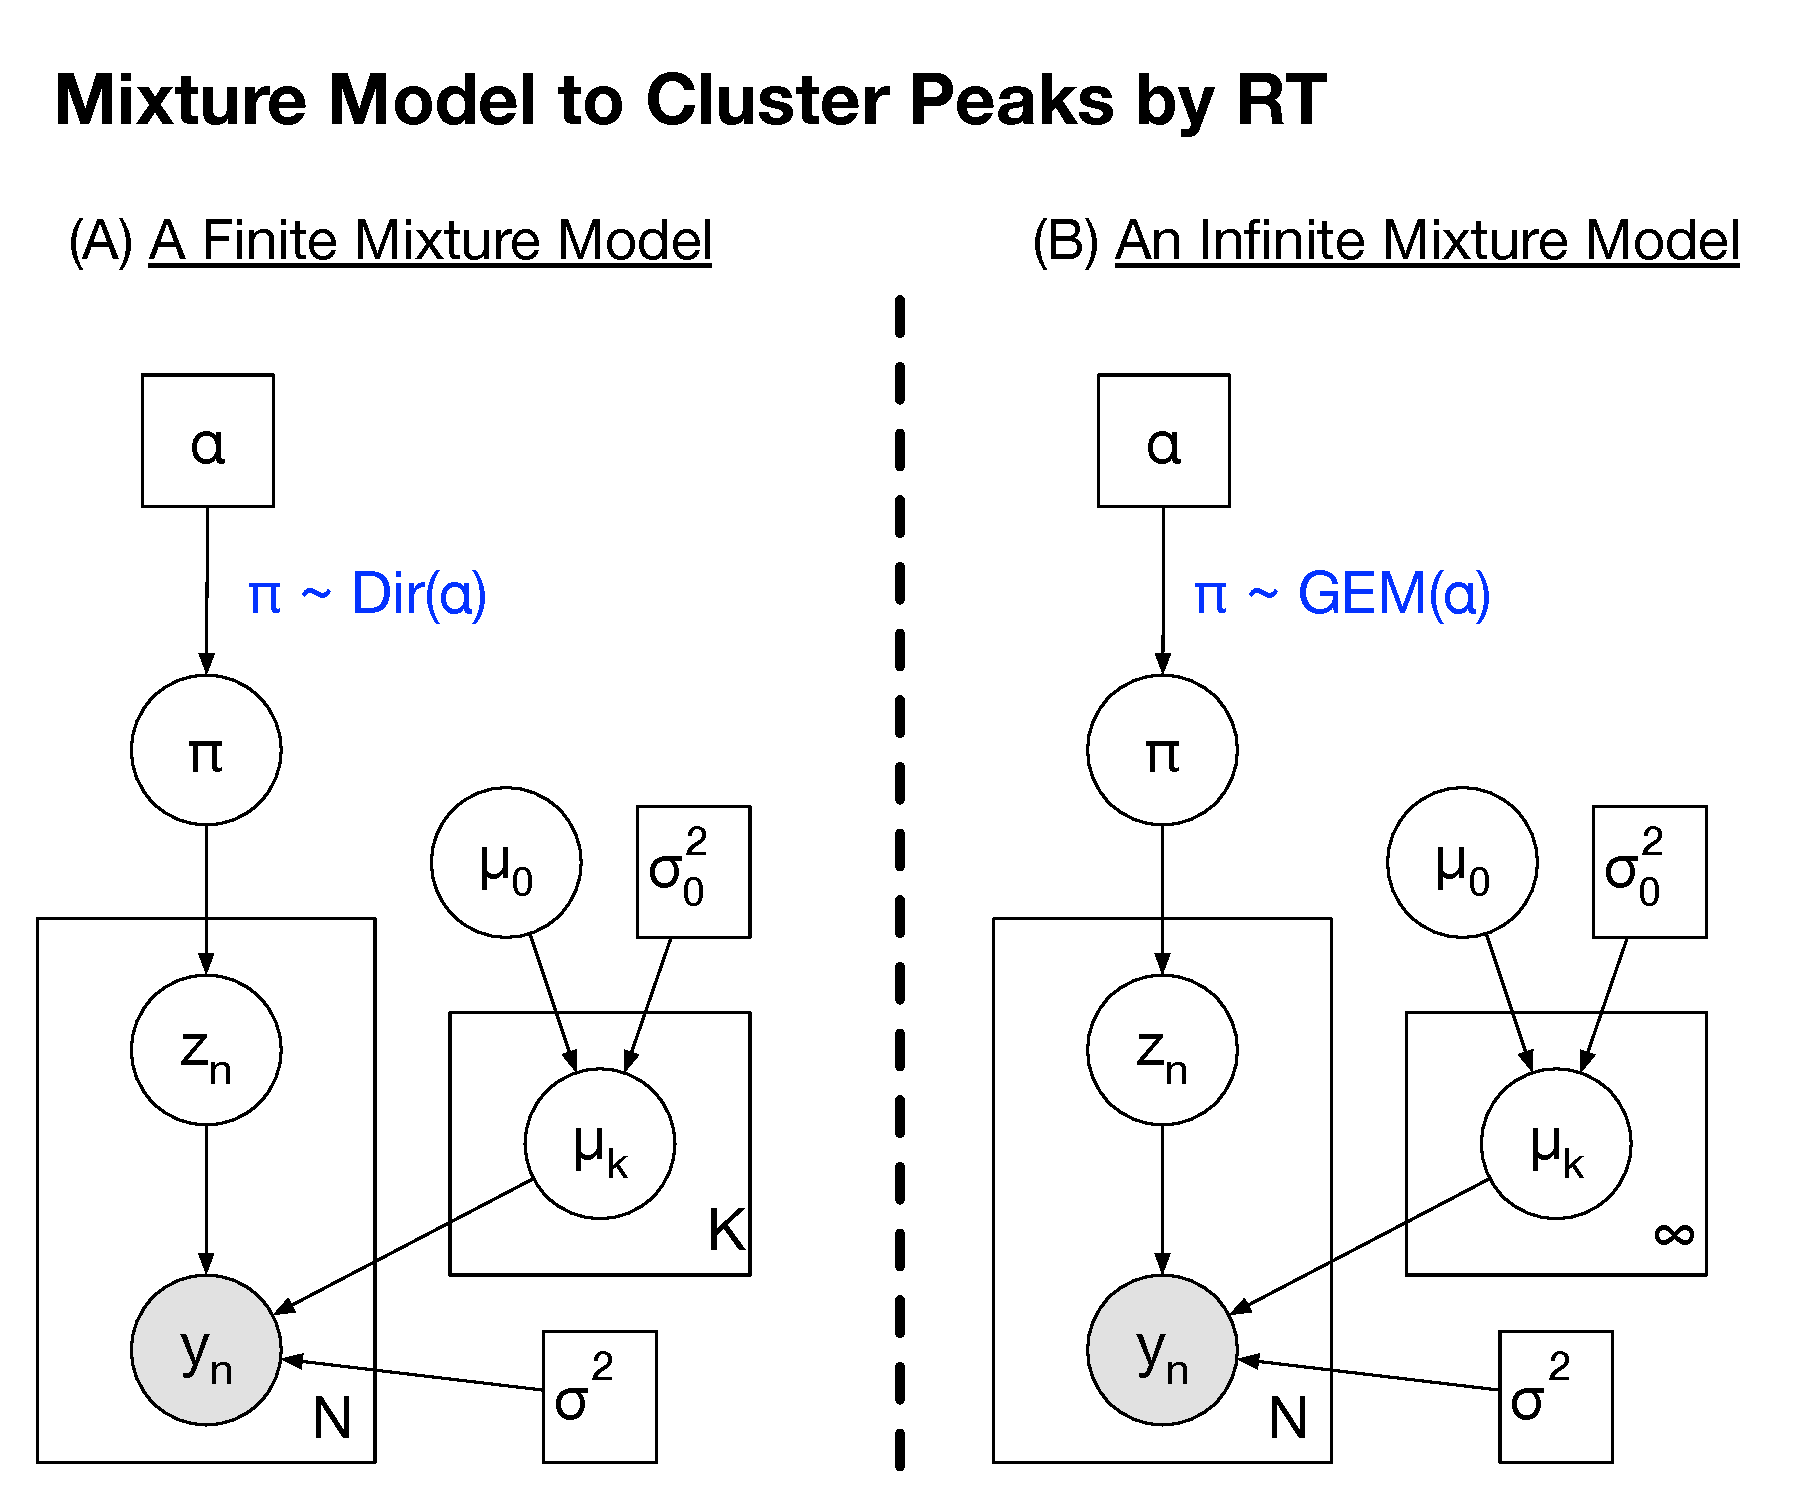
\includegraphics[width=0.8\textwidth]{03-machine-learning/figures/mixture_model.pdf}
\par\end{centering}
\caption{\label{fig:background-mixture-plate-diagram}Graphical models of (1) a finite mixture model, which is extended into (2) an infinite mixture model, to cluster peaks by their retention time (RT) values. Circles denotes random variables, squares denote fixed parameters, while the shaded node denotes an observed peak's RT.}
\end{figure}

We now explain the model specification in eq. (\ref{eq:background-finite-mixture}). First we assume that peaks that are related are generated by the same component in the mixture model. Let the variable $k=1,...,K$ index the mixture components. The choice of which probability distribution to use as a component is usually determined by the type of observed data. Each observed data point $y_n$ can be considered to a random variable drawn from the generating probability distribution. Assuming that each data point is generated by a univariate Gaussian distribution, we denote by $y_n \vert \mu, \sigma^2 \sim \mathcal{N}(\mu, \sigma^2)$ that $y_n$ is distributed as a Gaussian distribution having the mean $\mu$ and the variance $\sigma^2$ (as an alternative parameterisation, precision, i.e. the inverse variance ($\frac{1}{\sigma^2}$) can also be used, with a higher precision meaning a narrower distribution). The probability density function for this univariate Gaussian distribution is given by:
\begin{equation}
\mathcal{N}(y_n \vert \mu, \sigma^2) = \frac{1}{\sqrt{2\pi\sigma^2}}e^{-\frac{1}{2\sigma^2}(y_n-\mu)^2}
\end{equation}
For a single peak, its mixture model likelihood is therefore given by:
\begin{equation}
p(y_n \vert \boldsymbol{\mu},\boldsymbol{\pi}) = \sum_{k=1}^{K} \pi_k \mathcal{N}(y_n \vert \mu_k,\sigma^2)
\end{equation}
where $\pi_k$ is the mixture proportion (the positive weight for each component) and $\mu_k$ is mean for that component. $\boldsymbol{\pi}=\{\pi_{1},...,\pi_{k}\}$ denotes the vector over all mixture proportions that sums to one ($\sum_{k=1}^{K}\pi_{k}=1$). 

In this model, each mixture component is set to have an unknown mean $\mu_{k}$ but a known variance $\sigma^2$. The choice of setting an unknown $\mu_k$ but a fixed variance for $\sigma^2$ is motivated by the following reasonable modelling assumptions: \textbf{(1)} the retention time drift of observed peaks is broadly similar across the compounds being measured, and \textbf{(2)} this parameter can be set by the user based on his knowledge on the characteristic RT drifts of the LC instrument. Each cluster mean $\mu_k$ is assumed to be generated independently by a prior Gaussian distribution, parameterised by the mean $\mu_0$ and the variance $\sigma^2_0$. Let $\boldsymbol{\mu}=\{\mu_{1},...,\mu_{k}\}$ be the vector over all component means. This results in:
\begin{equation}
p(\boldsymbol{\mu} \vert \mu_0, \sigma^2_0) = \prod_{k=1}^K \mathcal{N}(\mu_k \vert \mu_0, \sigma^2_0)
\label{eq:background-prior-gaussian}
\end{equation}
We also require another random variable $z_{nk}$ to store the assignment of peak $n$ to cluster $k$, i.e. $z_{nk}=1$ if peak $n$ is assigned to cluster $k$ and 0 otherwise. Each peak is assumed to be generated independently by exactly one mixture component ($\sum_{k} z_{nk} = 1$). For a peak, its entire cluster assignments can be stored in a vector $\boldsymbol{z}_{n}$ of length $K$, where only $k$-th entry has a value of 1 (at $z_{nk}=1$). $\boldsymbol{z}_{n}$ is assumed to be generated from a multinomial distribution having the parameter vector $\boldsymbol{\pi}$. This multinomial distribution has the probability mass function given by:
\begin{equation}
\begin{aligned}
p(\boldsymbol{z}_n \vert \boldsymbol{\pi}) &= C \prod_{k=1}^{K} \pi_k^{z_{nk}}
\end{aligned}
\label{eq:background-zn_pmf}
\end{equation}
where $C$ is the multinomial coefficient, given by $\frac{(\sum_k z_{nk})!}{\prod_{k=1}^K z_{nk}!}$. Since $\boldsymbol{z}_{n}$ has only one draw from the multinomial, C evaluates to 1 and can be dropped. Now, let $\boldsymbol{Z}$ be the set of all indicator vectors for all peaks. This results in the following likelihood for all the peak assignment vectors:
\begin{equation}
\begin{aligned}
p(\boldsymbol{Z} \vert \boldsymbol{\pi}) &= \prod_{n=1}^N \prod_{k=1}^{K} \pi_k^{z_{nk}} \\
                                                              &= \prod_{k=1}^{K} \pi_k^{c_{k}}
\end{aligned}
\label{eq:background-z-given-pi}
\end{equation}
where $c_{k} = \sum_n z_{nk}$ is the count of peaks assigned to the $k$-th cluster. Collectively for all peaks, the joint likelihood of the observed data and the cluster assignments is:
\begin{equation}
p(\boldsymbol{y},\boldsymbol{Z}  \vert \boldsymbol{\mu},\boldsymbol{\pi}) = \prod_{n=1}^{N} \prod_{k=1}^{K} \big[ \pi_k \enspace \mathcal{N}(y_n \vert \mu_k,\sigma^2) \big]^{\boldsymbol{z}_{nk}}
\label{eq:background-mixture-likelihood}
\end{equation}

In our generative model, a prior distribution is also placed on $\boldsymbol{\pi}$. Due to its conjugacy to the multinomial distribution, a Dirichlet distribution parameterised by the vector $\boldsymbol{\alpha}=[\alpha_1,\alpha_2,...,\alpha_k]^T$ is a suitable prior. This results in:
\begin{equation}
\begin{aligned}
p(\boldsymbol{\pi} \vert \boldsymbol{\alpha}) &= \frac{\Gamma(\sum_{k} \alpha_{k})}{\prod_{k} \Gamma(\alpha_k)}  \prod_{k=1}^{K} \pi_k^{\alpha_{k}-1} \\
                                                                      &\propto \prod_{k=1}^{K} \pi_k^{\alpha_{k}-1}
\end{aligned}
\label{eq:background-pi-given-alpha}
\end{equation}

We can now state the complete joint likelihood of the model. Putting together the individual terms in eqs. (\ref{eq:background-prior-gaussian})-\ref{eq:background-pi-given-alpha}) and their respective independence assumptions, we obtain the joint probability distribution of the model parameters and data $p(\boldsymbol{y}, \boldsymbol{Z}, \boldsymbol{\mu}, \boldsymbol{\pi} \vert \boldsymbol{\alpha}, \allowbreak \mu_0,\sigma_0^2)$, which can be factorised into: 
\begin{equation}
p(\boldsymbol{y}, \boldsymbol{Z}, \boldsymbol{\mu}, \boldsymbol{\pi} \vert \boldsymbol{\alpha},\mu_0,\sigma_0^2) = p(\boldsymbol{y} \vert \boldsymbol{Z}, \boldsymbol{\mu},\boldsymbol{\pi}) p(\boldsymbol{Z} \vert \boldsymbol{\pi}) p(\boldsymbol{\pi} \vert \boldsymbol{\alpha}) p(\boldsymbol{\mu} \vert \mu_0, \sigma_0^2)
\label{eq:example-full-joint-dist}
\end{equation}

\subsection{Gibbs Sampling for a Finite Mixture Model}

Given the joint distribution in eq. (\ref{eq:example-full-joint-dist}), we are interested to infer the posterior distribution on the assignments $\boldsymbol{Z}$, the mixture proportions $\boldsymbol{\pi}$ and the cluster means $\boldsymbol{\mu}$. This is given by:
\begin{equation}
p(\boldsymbol{Z},\boldsymbol{\pi},\boldsymbol{\mu} \vert \boldsymbol{y}, \boldsymbol{\alpha},\mu_0,\sigma_0^2) = \frac{p(\boldsymbol{y}, \boldsymbol{Z}, \boldsymbol{\mu},\boldsymbol{\pi} \vert \boldsymbol{\alpha},\mu_0,\sigma_0^2)}{p(\boldsymbol{y} \vert \alpha,\mu_0,\sigma_0^2)}
\label{eq:background-mixture-posterior}
\end{equation}
Substituting eq. (\ref{eq:example-full-joint-dist}) into the numerator of eq. (\ref{eq:background-mixture-posterior}) results in the following posterior distribution over the parameters that we want to infer:
\begin{equation}
p(\boldsymbol{Z},\boldsymbol{\pi},\boldsymbol{\mu} \vert \boldsymbol{y},\alpha,\mu_0,s_0) \propto p(\boldsymbol{y} \vert \boldsymbol{Z}, \boldsymbol{\mu},\boldsymbol{\pi}) p(\boldsymbol{Z} \vert \boldsymbol{\pi}) p(\boldsymbol{\pi} \vert \boldsymbol{\alpha}) p(\boldsymbol{\mu} \vert \mu_0, s_0)
\label{eq:background-mixture-expanded-posterior}
\end{equation}

In many cases for the more interesting and complex models, the posterior distribution (such as the one in eq. \ref{eq:background-mixture-expanded-posterior}) and also the posterior predictive distribution cannot be derived analytically. Various methods, such as the EM algorithm \cite{gelman2014bayesian}, can be used to perform posterior inference in a mixture model, but throughout this thesis, we will use Gibbs sampling, an instance of Markov chain Monte Carlo (MCMC) methods. Gibbs sampling approximates the target posterior distribution by sequentially updating each random variable conditioned on all other random variables in the model. This requires deriving the \emph{conditional distribution} of each random variable that we want to infer. In some cases, obtaining these conditional distributions can be challenging, although the process can be simplified by the independence assumptions of our model (e.g. in assuming that the cluster means are independent) and through the use of the appropriate conjugate prior distributions.  Here we describe the steps required to construct a Gibbs sampler for the mixture model defined in eq. (\ref{eq:background-finite-mixture}).

As the initial step in our Gibbs sampler, we initialise the cluster means $\mu_1,\mu_2,..,\mu_k$ and the mixture proportion $\boldsymbol{\pi}$ by sampling from their respective prior distributions. Then we sequentially sample for new values of $\boldsymbol{Z}$, $\boldsymbol{\mu}$ and $\boldsymbol{\pi}$ from the conditional distributions listed below. 

\begin{enumerate}

\item We can update $\boldsymbol{z}_n$, the membership vector for peak $n$, by updating each of its $k$-th individual entry, i.e. $z_{nk}$. Simplifying eq. (\ref{eq:background-mixture-likelihood}) to consider just one $n$-th peak, we obtain the following after normalisation:
\begin{equation}
P(z_{nk}=1 \vert \boldsymbol{\pi}, y_n, \mu_k) = \frac{\pi_k \enspace \mathcal{N}(y_n \vert \mu_k, \sigma^2)}{\sum_{k=1}^K \pi_k \enspace \mathcal{N}(y_n \vert \mu_k, \sigma_2)}
\label{eq:background-mixture-conditional-z}
\end{equation}

\item As the next step, we also need to update each $\mu_k$ conditioned on the membership vectors $\boldsymbol{Z}$ and the hyperparameters $\mu_0$ and $\sigma_0$. Consider one $k$-th cluster, and let $\boldsymbol{x}_k=\{x_1, x_2, ..., x_m\}$ be the set of peaks currently assigned to cluster $k$. The variable $m$ indexes over the member peaks of cluster $k$, and there are $M_k$ such peaks. Their joint likelihood is given by $p(\boldsymbol{x}_k \vert \mu_k)$. As defined in eq. (\ref{eq:background-prior-gaussian}), we assume that each $\mu_k$ is independent given its conjugate prior $\mathcal{N}(\mu_0, \sigma_0^2)$ . The posterior distribution on $p(\mu_k \vert \boldsymbol{x}_k, \mu_0)$ is therefore:
\begin{equation}
\begin{aligned}
p(\mu_k \vert \boldsymbol{x}_k, \mu_0) &\propto p(\boldsymbol{x}_k \vert \mu_k) \cdot p(\mu_k \vert \mu_0) \\
                                                              &= \prod_{m=1}^{M_k} \mathcal{N}(x_m \vert \mu_k, \sigma^2) \cdot \mathcal{N}(\mu_k \vert \mu_0, \sigma_0) \\
                                                           &= \prod_{m=1}^{M_k} \frac{1}{\sqrt{2\sigma^2\pi}} exp\bigg(\frac{-(x_n-\mu_k)^2}{2\sigma^2} \bigg) \cdot \frac{1}{\sqrt{2\sigma_0^2\pi}} exp\bigg(\frac{-(\mu_k-\mu_0)^2}{2\sigma_0^2} \bigg)
\end{aligned}                                                           
\label{eq:background-posterior_mu_k}
\end{equation}
Since $p(\mu_k \vert \boldsymbol{x}_k, \mu_0)$ is a product of Gaussians, the posterior is proportional to another Gaussian, parameterised by say $\mathcal{N}(\tilde{\mu}, \tilde{\sigma}^2)$. Equating this with eq. (\ref{eq:background-posterior_mu_k}) results in:
\begin{equation}
exp\bigg(\frac{-(\mu_k-\tilde{\mu})^2}{2\tilde{\sigma}^2} \bigg) \propto exp\bigg(\frac{-\sum_{m=1}^{M} (x_m-\mu_k)^2}{2\sigma^2} + \frac{-(\mu_k-\mu_0)^2}{2\sigma_0^2}\bigg)
\label{eq:background-solving-posterior-mu_k}
\end{equation}
Simplifying eq. (\ref{eq:background-solving-posterior-mu_k}) and completing the squares, we obtain the following parameters for $\mathcal{N}(\mu_k \vert \tilde{\mu}, \tilde{\sigma}^2)$:
\begin{equation}
\tilde{\mu} = \tilde{\sigma}^2 \bigg( \frac{\sum_{m=1}^{M} x_m}{\sigma^2} + \frac{\mu_0}{\sigma_0^2} \bigg), \enspace
\tilde{\sigma}^2 = \frac{1}{\frac{M}{\sigma^2} + \frac{1}{\sigma^2_0}} 
\label{eq:background-tilde-mu-sigma}
\end{equation}

\item Finally we also need to update the mixture proportion $\boldsymbol{\pi}$. Putting together the multinomial likelihood and Dirichlet prior in eqs. (\ref{eq:background-z-given-pi}) and (\ref{eq:background-pi-given-alpha}), we obtain a conditional distribution for $\boldsymbol{\pi}$ that is another Dirichlet distribution, parameterised by $[\alpha_{1}+c_{1}, \alpha_{2}+c_{2}, ..., \alpha_{k}+c_{k}]^T$. Each entry in this parameter vector is influenced by two values: the pseudo-count contribution from $\alpha_k$ and the actual counts of peaks currently assigned to cluster $k$ from $c_k$. 
\begin{equation}
\begin{aligned}
p(\boldsymbol{\pi} \vert \boldsymbol{\alpha}, \boldsymbol{Z}) = p(\boldsymbol{Z} \vert \boldsymbol{\pi}) \cdot p(\boldsymbol{\pi} \vert \boldsymbol{\alpha})
                                                                                                &\propto \prod_{k=1}^{K} \pi_k^{\alpha_{k}-1} \cdot \prod_{k=1}^{K} \pi_k^{c_{k}}  \\
                                                                                                &= \prod_{k=1}^{K} \pi_k^{\alpha_{k}+c_{k}-1} \\
                                                                                                &= Dir(\alpha_{1}+c_{1}, \alpha_{2}+c_{2}, ..., \alpha_{k}+c_{k})
\end{aligned}
\label{eq:background-mixture-conditional-pi}
\end{equation}

\end{enumerate}

In Gibbs sampling, each newly updated value is immediately used before sampling for the next value. This sampling of each random variable is repeated until convergence. Often a certain number of initial samples are discarded during the \emph{burn-in} period. Since successive samples are correlated, a certain \emph{thinning} interval is also used to reduce the number of samples used. The resulting samples can now be used to approximate the true posterior distribution of the model. Frequently, the marginal distribution of the random variable of interest is studied. Particularly for our case, often we are interested in the probability of any pair of peaks (or even a set of peaks) to be placed in the same component since, as the subsequent chapters will show, this has a direct application to the problem of peak alignment.

\subsection{Collapsed Gibbs Sampling for a Finite Mixture Model}

As we have chosen conjugate prior distributions on the mixture proportion $\boldsymbol{\pi}$ and also the cluster mean $\mu_k$, it is possible for us to integrate (\emph{collapse}) $\boldsymbol{\pi}$ and $\mu_k$ from the model during Gibbs sampling. This results in a collapsed Gibbs sampler (CGS) where we need not sample $\boldsymbol{\pi}$ and $\mu_k$ explicitly. Collapsing has also been shown to lead to a better model convergence \cite{gelman2014bayesian}. It will also help in the next section when we want to extend our finite mixture model (where $K$ the number of components is specified) to an infinite mixture model (where the number of components is unbounded) as we do not need to explicitly sample an infinite-dimensional vector $\boldsymbol{\pi}$. 

Specifically in this CGS implementation, we aim to marginalise $\boldsymbol{\pi}$ and $\mu_k$ by integrating them out from the conditional probability for $z_{nk}$, the assignment of peak $n$ to cluster $k$. Collapsing $\boldsymbol{\pi}$ introduces dependencies among all the $\boldsymbol{z}_n$ random variables, so we introduce another notation $\boldsymbol{Z}^{-}$ to mean all other $\boldsymbol{z}_n$s except the one for the current $n$-th peak being sampled upon. Similarly, $\boldsymbol{y}^{-}$ denotes the RT values for other peaks apart from $y_n$. The conditional distribution for $z_{nk}$ in the CGS is given by:
\begin{equation}
\begin{aligned}
p(z_{nk}=1, \boldsymbol{\pi} \vert \boldsymbol{Z}^{-}, \boldsymbol{y}, \mu_0, \boldsymbol{\alpha}) \propto p(y_n \vert \boldsymbol{Z}^{-},  \boldsymbol{y}^{-}, \mu_0) \cdot P(z_{nk}=1 \vert \boldsymbol{Z}^{-}, \boldsymbol{\alpha})
\end{aligned}
\label{eq:background-collapsed-gibbs}
\end{equation}
We consider both terms of eq. (\ref{eq:background-collapsed-gibbs}) separately. 
\begin{enumerate}

\item The first term on the right hand side of eq. (\ref{eq:background-collapsed-gibbs}) is the likelihood of $y_n$ to be assigned to cluster $k$. Here, we no longer need to sample for $\mu_k$ as we are integrating over all values of $\mu_k$ using the posterior distribution $\mathcal{N}(\mu_k \vert \tilde{\mu}, \tilde{\sigma}^2)$ defined in eq. (\ref{eq:background-solving-posterior-mu_k}). Instead we can directly compute this likelihood by:
\begin{equation}
\begin{aligned}
p(y_n \vert \boldsymbol{Z}^{-},  \boldsymbol{y}^{-}, \mu_0) &\propto \int p(y_n \vert \mu_k) \cdot p(\mu_k \vert \boldsymbol{Z}^{-},  \boldsymbol{y}^{-}, \mu_0) \enspace d\mu_k \\
                                                                                            &\propto \int \mathcal{N}(y_n \vert \mu_k, \sigma^2) \cdot \mathcal{N}(\mu_k \vert \tilde{\mu}, \tilde{\sigma}^2) \enspace d\mu_k \\
                                                                                            &\propto \mathcal{N}(y_n \vert \tilde{\mu}, \sigma^2 + \tilde{\sigma}^2)
\end{aligned}
\label{eq:background-tilde-mu-sigma-variance}
\end{equation}
where $\tilde{\mu}$ and $\tilde{\sigma}$ are defined in eq. (\ref{eq:background-tilde-mu-sigma}). 

As an alternative parameterisation, we can also rewrite $\tilde{\mu}$ and $\tilde{\sigma}^2$ using precision (inverse variance) $\tau=\frac{1}{\sigma^2}$ and $\tau_0=\frac{1}{\sigma_0^2}$ to replace the variances. The expression in eq. (\ref{eq:background-tilde-mu-sigma}) then becomes:
\begin{equation}
\begin{aligned}
\tilde{\mu}     &= \tilde{\sigma}^2 \bigg( \frac{\sum_{m=1}^{M} x_m}{\sigma^2} + \frac{\mu_0}{\sigma_0^2} \bigg) = \frac{\tau\sum_{m=1}^{M} x_m + \mu_0\tau_0}{M\tau + \tau_0} \\
\tilde{\sigma} &= \frac{1}{\frac{M}{\sigma^2} + \frac{1}{\sigma^2_0}} = \frac{1}{M\tau + \tau_0}
\label{eq:background-tilde-mu-sigma-precision}
\end{aligned}
\end{equation}
In the Gibbs samplers for the mixture models in the later chapters, this parameterisation using precision is what we will use.

\item The second term on the right hand side of eq. (\ref{eq:background-collapsed-gibbs}) is the prior probability of assigning the $n$ peak to cluster $k$. Again we do not have to sample for $\boldsymbol{\pi}$ as we integrate over all values of $\boldsymbol{\pi}$. Our desired conditional probability is given in eq. (\ref{eq:background-integrated-pi}). By definition, $P(z_{nk}=1 \vert \boldsymbol{\pi})$ is $\pi$ while $p(\boldsymbol{\pi} \vert \boldsymbol{Z}^{-}, \boldsymbol{\alpha})$ is the posterior Dirichlet defined in eq. (\ref{eq:background-mixture-conditional-pi}). This results in:
\begin{equation}
\begin{aligned}
P(z_{nk}=1 \vert \boldsymbol{Z}^{-}, \boldsymbol{\alpha}) &= \int P(z_{nk}=1 \vert \boldsymbol{\pi}) \cdot p(\boldsymbol{\pi} \vert \boldsymbol{Z}^{-}, \boldsymbol{\alpha}) \enspace d\boldsymbol{\pi} \\
                                                                                         &= \frac{c_k + \alpha_k}{\sum_{k=1}^K c_{k} + \alpha_k}
\label{eq:background-integrated-pi}
\end{aligned}
\end{equation}
A derivation for the integral in eq. (\ref{eq:background-integrated-pi}) can be found in Ch. 24 of \cite{murphy2012machine}. In the result of eq. (\ref{eq:background-integrated-pi}), $c_{k}$ denotes the number of data points (peaks) currently assigned to cluster $k$,  excluding the $n$-th peak that is being sampled. 

Eq. (\ref{eq:background-integrated-pi}) reveals the clustering property of the Dirichlet-multinomial mixture model. The larger a $k$-th cluster is, the greater the prior probability for the currently sampled peak to be placed into that cluster. This is balanced by the prior hyperparameter $\alpha_k$. In the absence of any prior knowledge, often $\alpha_k$ is set to be symmetric ($\alpha_k=\frac{\alpha}{K})$, and in this case, small values for $\alpha_k$ will result in fewer, larger clusters as $c_k$ dominates, while large values for $\alpha_k$ will smoothen the prior probabilities, reducing the influence of $c_k$ and producing more uniform clusters. In this manner, $\alpha_k$ plays the role of the pseudo-count that controls how strong the influence of $c_k$ is. 
\end{enumerate}

Having derived the terms in the conditional distribution for $z_{nk}$, we can now describe our CGS for this mixture model. We loop over each peak in a random order and remove the information of that peak from the model. We then resample the assignment of peak $n$ to each of the $K$ clusters using eq. (\ref{eq:background-collapsed-gibbs}), normalised to form a probability distribution. Upon sampling a new cluster ($z_{nk}=1$), we assign peak $n$ to cluster $k$ and add the information of that peak back into the model. This consists of one iteration in our CGS. Each iteration generates a sample, and the collection of samples can be used to approximate our posterior model parameters.

\section{Dirichlet Process Mixture Model Clustering\label{background-dp-clustering}}

One parameter that has to be specified in the model is $K$, the number of mixture components. However, in many cases, often we do not know the number of components in advance. Determining the number of clusters in general is a challenging problem. In the Bayesian context, selecting $K$ (and also other model parameters) constitute the model selection process. Bayesian non-parametric approach provides a way to perform model selection on the number of mixture components in a principled manner by assuming that there is an infinite set of parameters, but the observed data is generated from a finite subset of that. In this manner, for the non-parametric clustering approach, we do not specify the number of cluster $K$ \emph{a-priori } but instead assume that the data is generated from a mixture of an infinite number of components. The non-parametric clustering model then learns the number of clusters from the data, allowing for the automatic determination of model complexity \cite{hjort2010bayesian}.

Dirichlet Process (DP) \cite{ferguson1973bayesian} is a stochastic process that describes a distribution over probability measures, often used in Bayesian non-parametric mixture model to generate the prior distributions over the mixture components when the number of component is unknown. Here, we focus on providing a brief overview on Dirichlet Process to use in the construction of an infinite mixture model. For more details, the reader is referred to \cite{murphy2012machine, Rasmussen2000, hjort2010bayesian,teh2011dirichlet}. The DP is parameterised by a base distribution $H$ and a concentration parameter $\alpha$, i.e. $DP(H, \alpha)$. A constructive definition for the DP is given through the stick-breaking construction \cite{ishwaran2011gibbs}. Let $\boldsymbol{\pi}$ be an infinite-dimensional mixture proportion vector, consisting of the following infinite sequence of entries $\boldsymbol{\pi}=\{\pi_1, \pi_2, ..., \}$. Then $\boldsymbol{\pi} \sim GEM(\alpha)$, where GEM stands for the Griffiths, Engen and McCloskey distribution, if we can generate the $k$-th entry in $\boldsymbol{\pi}$ with the following stick-breaking process:
\begin{equation}
\begin{aligned}
\beta_k &\sim Beta(1, \alpha) \\
\pi_k     &= \beta_k \prod_{l=1}^{k-1} (1-\beta_l) 
\end{aligned}
\label{eq:background-stick-breaking-construction}
\end{equation}
To use eq. (\ref{eq:background-stick-breaking-construction}), first we see that expanding the expression for $\pi_k$ in eq. (\ref{eq:background-stick-breaking-construction}) results in the following recursive definition, where each $\pi_k$ is a product of $\beta_k$ and $(1-\sum_{l=1}^{k-1} \pi_l)$.
\begin{equation}
\begin{aligned}
\pi_1 &= \beta_1 \\
\pi_2 &= \beta_2(1-\beta_1) \\
\pi_3 &= \beta_3(1-\beta_2)(1-\beta_1) \\
         &= \beta_3(1-\beta_1-\beta_2(1-\beta_1)) \\
         &= \beta_3(1-\pi_1-\pi_2) \\
... \\
\pi_k &= \beta_k(1-\sum_{l=1}^{k-1} \pi_l)
\end{aligned}
\label{eq:background-pi-gem}
\end{equation}
So to start the stick-breaking process, we begin with a stick of length 1 and generate a random variable $\beta_1 \sim Beta(1, \alpha)$. This random variable $\beta_1$ is used to define the position to break the stick initially at $\pi_1 = \beta_1$. We repeat infinitely the step of generating a new $\beta_k \sim Beta(1, \alpha)$ and using it to break the remaining portion of the stick $(1-\sum_{l=1}^{k-1} \pi_l)$ at $\pi_k$. The result of this process is a vector $\boldsymbol{\pi}$ that is Dirichlet-distributed. It can be shown that $\sum_{k=1}^{\infty} \pi_k=1$ \cite{ishwaran2011gibbs}. The stick-breaking process defines an exchangeable distribution: although parts of the sticks are generated in order and each part is conditioned on the previous ones, the resulting joint distribution is independent of the order.

In the mixture setting, $\boldsymbol{\pi}$ generated in this manner can be used as the mixture proportions in an infinite mixture model. Instead of sampling a finite-length vector from the Dirichlet distribution in eq. (\ref{eq:background-finite-mixture}), we generate $\boldsymbol{\pi}$ from the stick-breaking process. This lets us formulate the generative process for our data as a mixture model having infinitely-many mixture components using the stick-breaking construction as the prior over $\boldsymbol{\pi}$, resulting in the graphical model shown in Figure~\ref{fig:background-mixture-plate-diagram}B. This also lets us specify an infinite mixture model in term of samples from the Dirichlet Process. Given $\boldsymbol{\pi}$ generated as before and a base distribution $H$ that we can sample from, let $\phi_k$ be a value sampled from $H$ (this can be, for instance, the mean $\mu_k$ of a mixture component). Then the following $G$ is a discrete distribution that is also an infinite mixture model:
\begin{equation}
G=\sum_{k=1}^{\infty} \pi_k \delta_{\phi_k}
\end{equation}
where $\delta_{\phi_k}$ is the delta function that has its entire probability distribution concentrated at $\phi_k$. We say that $G \sim DP(\alpha, H)$ is a sample from the Dirichlet Process parameterised by the concentration parameter $\alpha$ and the base distribution $H$ \cite{teh2011dirichlet}. In this manner, the DP is a distribution over distributions. A sample from the DP is a discrete probability distribution, even if the base distribution $H$ is continuous. The level of this discretisation is controlled by $\alpha$. Small $\alpha$ results in a distribution concentrated at fewer discrete values, while large $\alpha$ produces a distribution with support over many discrete values.

An alternative formulation of an infinite mixture model can be given using a DP parameterised by $\alpha$ and the base distribution $H=\mathcal{N}(\mu_0, \sigma_0^2)$. With a fixed variance ($\sigma^2$) that represents a user-defined RT drift tolerance, the generative process for our peak RT data becomes:
\begin{equation}
\begin{aligned}
G \vert \alpha, H  &\sim DP(\alpha, H) \\
\mu_k \vert G     &\sim G \\
y_n \vert \mu_k  &\sim \mathcal{N}(y \vert \mu_k, \sigma^2)
\end{aligned}
\label{eq:background-infinite-mixture-dp}
\end{equation}

\begin{figure}
\noindent \begin{centering}
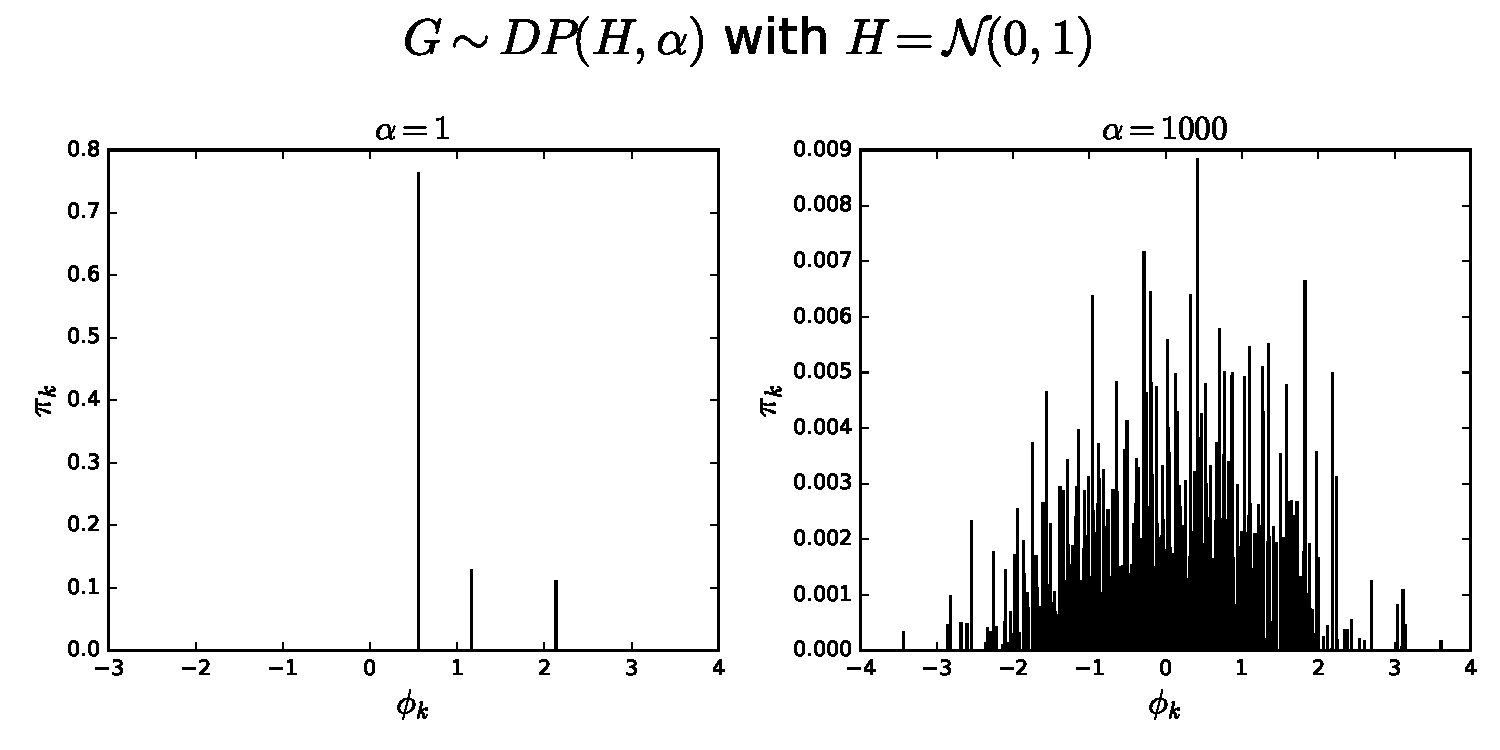
\includegraphics[width=1.0\textwidth]{03-machine-learning/figures/dp_samples_stick.pdf}
\par\end{centering}
\caption{\label{fig:g-from-dp-stick}Two samples of $G$, plotted up to 1000 discrete values, generated by a Dirichlet Process with $\alpha=1$ (left) and $\alpha=1000$ (right) and a base distribution $\mathcal{N}(0, 1)$. We see that $\alpha$ affects how smooth the resulting discretisation of $H$ is in $G$.}
\end{figure}

Figure~\ref{fig:g-from-dp-stick} shows two examples of $G$ drawn from a DP with a Gaussian base distribution, $H=\mathcal{N}(0, 1)$ and varying values for $\alpha$. As noted earlier, a key property of the DP is that $G$ is a discrete distribution despite $H$ being continuous. The level of discretisation of $H$ is controlled by $\alpha$, with small $\alpha$ resulting in fewer discrete points with larger probabilities in $G$ and large $\alpha$ causing $G$ to have more discrete points. Repeated sampling from $G$ will generate repeated values, which illustrates the usefulness of the DP, in particular for clustering by setting the DP as a prior over the distribution of the mixture components. 

We also show in Figure~\ref{fig:g-from-dp} how the generative process in eq. (\ref{eq:background-infinite-mixture-dp}) works. First we sample a distribution $G$ from the DP parameterised by $\alpha$ and a base distribution $H$. In the example of Figure~\ref{fig:g-from-dp}A, the base is set to $\mathcal{N}(0, 1)$ and $G$ contains two unique discrete values, denoted by the red and green crosses, each of which is also a cluster component mean $\mu_k$. Every $n$-th data point is associated with a $\mu_k$, and each $\mu_k$ generates the data for its cluster by sampling for values from $\mathcal{N}(\mu_k, \sigma^2)$. 
\begin{figure}
\noindent \begin{centering}
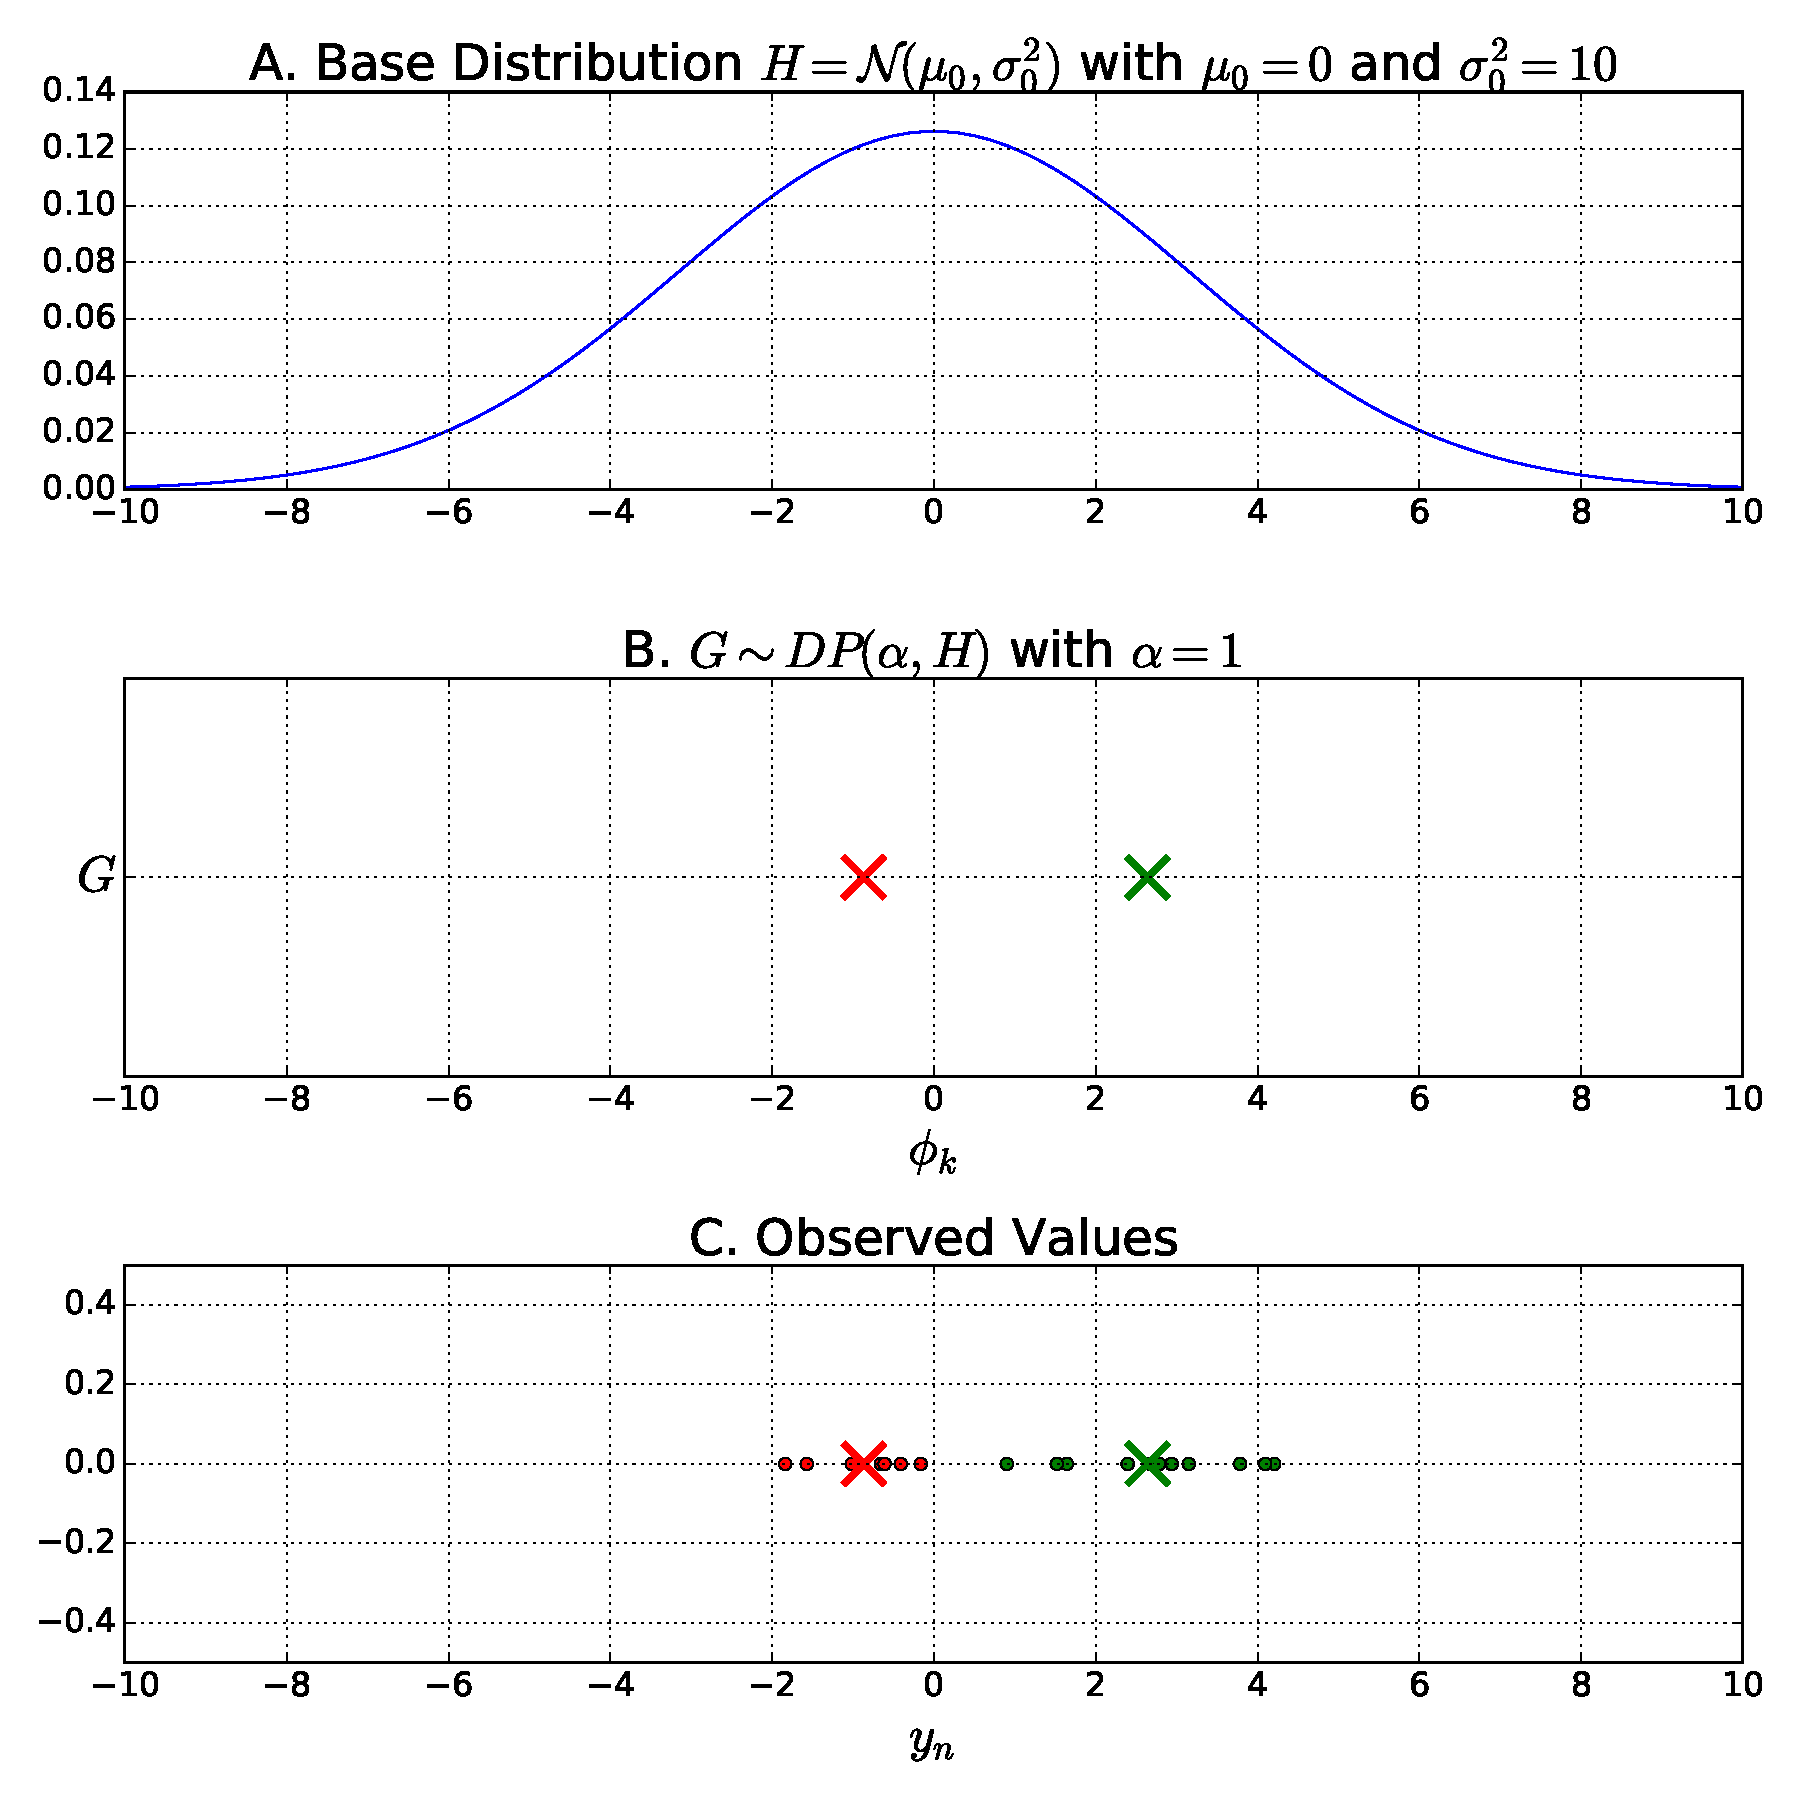
\includegraphics[width=0.6\textwidth]{03-machine-learning/figures/dp_samples.pdf}
\par\end{centering}
\caption{\label{fig:g-from-dp}An illustration of the generative process for the DP mixture model in eq. (\ref{eq:background-infinite-mixture-dp}). First, we require a base distribution to sample for discrete values, shown in \textbf{(A)}. Given $H$ and some concentration parameter $\alpha$, we generate a discrete distribution $G$. In \textbf{(B)}, we see that $G$ contains two unique discrete values sampled from $H$, represented by the red and green crosses. Each discrete value in G $\phi_k$ is also a cluster mean $\mu_k$. \textbf{(C)} The noisy observed values is generated by sampling for $\mu_k$ from $G$, and sampling for $y_n$ conditioned on the $\mu_k$.}
\end{figure}

\subsection{Collapsed Gibbs Sampling for a Dirichlet Process Mixture Model \label{background-cgs-dpmixture}}

Having defined the generative process for an infinite mixture model, we are now interested in performing inference on the model parameters. In particular for Gibbs sampling, we require the probability of the current $n$-th data point that is being sampled to be in a cluster ($P(z_{nk}=1$), conditioned on the assignments of other data points ($\boldsymbol{Z}^{-}$). We show how we derive this by modifying the original collapsed Gibbs sampler as the number of components $K$ goes to infinity. Assuming a symmetric prior on the Dirichlet hyperparameter, $\alpha_k=\frac{\alpha}{K}$, then the conditional probability on the assignment of peak $n$ to cluster $k$ from eq. (\ref{eq:background-integrated-pi}) becomes:
\begin{equation}
P(z_{nk}=1 \vert \boldsymbol{Z}^{-}, \boldsymbol{\alpha}) = \frac{c_k + \frac{\alpha}{K}}{\alpha+N-1}
\label{eq:background-integrated-pi-symmetric}
\end{equation}
As before, $c_k$ in eq. (\ref{eq:background-integrated-pi-symmetric}) refers to the count of the number of peaks assigned to cluster $k$, excluding the current one being sampled. In the denumerator of eq. (\ref{eq:background-integrated-pi-symmetric}), we also see $\alpha+N-1$ instead of just $\alpha+N$ to exclude the current data point being sampled in this iteration of Gibbs sampling. Then taking the limit of eq. (\ref{eq:background-integrated-pi-symmetric}) as $K$ goes to infinity results in the following conditional probability for $z_{nk}=1$:
\begin{equation}
P(z_{nk}=1 \vert \boldsymbol{Z}^{-}, \boldsymbol{\alpha}) = 
\begin{cases}
    \frac{c_k}{\alpha+N-1}, & \text{for existing clusters} \\
    \frac{\alpha}{\alpha+N-1}, & \text{for a new cluster}
\end{cases}
\label{eq:background-crp}
\end{equation}
The conditional probability in eq. (\ref{eq:background-crp}) is also often formulated as the Chinese Restaurant Process (CRP) \cite{frigyik2010introduction}. In this process, an analogy is proposed based on a Chinese restaurant having an infinite number of tables. Tables correspond to clusters while customers correspond to the observed data points. The CRP is a random process that defines the probability of a customer to sit at a particular table, conditioned on the seating arrangements of other customers. For a non-empty table, this probability is proportional to $c_k$, the number of other customers seated at a table, while for an empty table, the probability is proportional to $\alpha$. Under exchangeablity, the joint posterior distribution in the CRP is invariant to the ordering of the items \cite{aldous1985exchangeability}. This means we can assume that the $n$-th data point is the last customer to arrive in the CRP, and the conditional probability for $P(z_{nk}=1)$ is thus proportional to eq. (\ref{eq:background-crp}). Coupled with a likelihood for a data point to be assigned to a table, we can use this to modify our conditional probability for Gibbs sampling, resulting in:
\begin{equation}
P(z_{nk}=1 \vert \boldsymbol{Z}^{-}, \boldsymbol{\alpha}) \propto 
\begin{cases}
    c_k \cdot p(y_n \vert \boldsymbol{Z}^{-},  \boldsymbol{y}^{-}, \mu_0) \\
    \alpha \cdot p(y_n \vert \mu_0)
\end{cases}
\label{eq:background-infinite-mixture-model-sampling}
\end{equation}
The top term in eq. (\ref{eq:background-infinite-mixture-model-sampling}) corresponds to the probability of being assigned to existing non-empty clusters. As in the finite mixture model case, this prior probability is proportional to $c_k$, the number of data points (peaks) currently assigned to cluster $k$ excluding the $n$-th peak that is being sampled, while the likelihood $p(y_n \vert \boldsymbol{Z}^{-},  \boldsymbol{y}^{-}, \mu_0)$ is defined in eq. (\ref{eq:background-tilde-mu-sigma-variance}) or equivalently in eq. (\ref{eq:background-tilde-mu-sigma-precision}) when precision is used. The bottom term in eq. (\ref{eq:background-infinite-mixture-model-sampling}) corresponds to the probability of creating a new cluster with the prior probability proportional to $\alpha$ multiplied by the data likelihood. In this particular case due to conjugacy, we can derive $p(y_n \vert \mu_0)$, the likelihood of $y_n$ conditioned on the hyperparameter mean $\mu_0$ directly by marginalising over all empty components, resulting in:
\begin{equation}
\begin{aligned}
p(y_n \vert \mu_0) &= \int p(y_n \vert \mu_k) p(\mu_k \vert \mu_0) \enspace d_{\mu_k}
                               &= \mathcal{N}(y_n \vert \mu_0, \sigma^2 + \sigma_0^2)
\end{aligned}
\label{eq:background-new-table-likelihood}
\end{equation}
In other cases where it is not possible to derive the data likelihood analytically, we can approximate it by sampling for a new $\mu_k$ from the prior instead and evaluating $y_n$ under the new cluster mean \cite{Rasmussen2000}. This completes the necessary modification to our collapsed Gibbs sampler. The sampling process proceeds largely as before by removing the $n$-th peak from the model and performing the assignment of that peak to cluster $k$ using eq. (\ref{eq:background-infinite-mixture-model-sampling}). If an existing $k$ is selected, this is then the same as the finite mixture case. When a new $k$ is selected, we create a new cluster and assign the peak to that cluster. In this manner, the number of mixture components is not fixed in advance \textit{a priori}, but is instead determined based on the observed data and the choice of hyperparameter $\alpha$.

\section{Hierarchical Dirichlet Process Mixture Model Clustering\label{background-hdp-clustering}}

While the DP mixture model allows us to cluster related peaks together, the clustering process within each run is performed separately and independently of the others. However, in some cases it is useful to allow for clustering to be shared across runs. We call the clusters shared in this manner to be the \emph{global clusters}, as opposed to the \emph{local clusters} that are found in each file. In LC-MS data, global clusters can be assumed to correspond to compounds (e.g. metabolites or peptide fragments) that are present in all runs, while local clusters are the noisy realisation of such global clusters in each run. Often, the shared presence of global clusters can be assumed when we have multiple runs generated from the measurements of the same biological sample. In this case, the runs are called technical replicates. In other circumstances when the runs are generated through the measurements of different biological samples, shared compounds might also be found and can therefore be represented as global clusters.

Hierarchical Dirichlet Process (HDP) mixture model is an extension of the DP mixture model that allows for such global clusters to be defined and shared across multiple runs \cite{teh2005hierarchical,teh2012hierarchical}. Within each file, the observed data points are clustered into local clusters, which are assigned to the shared global clusters. In our application, the HDP mixture model is particularly useful for alignment as being able to generatively explain which peaks are generated by which global clusters is the same as being able to match these peaks across runs. This application is shown in Chapter~\ref{c:hdp} where we introduce a HDP mixture model to simultaneously group peaks within and across runs. From the model, the matching of peaks (alignment) is constructed from the marginal probabilities of peaks of being assigned into the same global cluster. 

To understand the HDP mixture model, first we need to define the hierarchical Dirichlet Process. Given a concentration parameter $\alpha_0$ and a base distribution $H$, let $G_0$ to be a distribution sampled from a $DP(\alpha_0, H)$. Then for each file $j=1,...J$, we can sample a file-specific distribution $G_j$ from another Dirichlet Process parameterised by $\alpha_j$, with $G_0$ as its base distribution. This file-specific DP is denoted as $DP(\alpha_j, G_0)$, resulting in:
\begin{equation}
\begin{aligned}
G_0 \vert \alpha_0, H &\sim DP(\alpha_0, H) \\
G_j \vert \alpha_j, G_0 &\sim DP(\alpha_j, G_0)
\end{aligned}
\label{eq:background-hdp-process}
\end{equation}
As a property of the DP, $G_0$ is a discrete distribution with probabilities that sums to 1 (regardless of whether $H$ is continuous or discrete). This means $G_0$ has a support over the discrete values ${\phi_1, \phi_2, ... }$ drawn from its base distribution $H$. We use $G_0$ to represent the prior distribution over the global clusters. Each $G_j$ is a prior distribution over the file-specific local clusters, and since $G_j$ is drawn from a DP with $G_0$ as its base distribution, each $G_j$ is discrete and has a support over the same discrete values as $G_0$. This is where the sharing property of the HDP comes about. The set of discrete values in $G_0$, which represent the prior values on the global clusters, are inherited (copied) to be the discrete values in $G_j$, which represents represent the prior values on the local clusters.

To define a HDP mixture model, we complete the hierarchical prior defined in eq. (\ref{eq:background-hdp-process}) with a data-generating distribution. Continuing with our example of clustering peaks by their RT values, the data now comes in $J$ input files, each corresponding to an LC-MS run. Let $j=1,...,J$ indexes over the input files, while $n=1,...,N$ indexes over the peaks in a particular $j$-th file. Within a $j$-th file, the observed data is $\boldsymbol{y}_j=\{y_{j1}, y_{j2}, ..., y_{jn}\}$. We assume that within a file, the noise on the observed RT values is generated by a Gaussian with mean $\mu_{jk}$ and a fixed variance $\sigma^2$. As the base distribution, we set $H=\mathcal{N}(\mu_0, \sigma_0^2)$. Together with the prior in eq. (\ref{eq:background-hdp-process}), we obtain the following HDP mixture model that explains how the RT values of peaks in multiple files can be generated:
\begin{equation}
\begin{aligned}
G_0 \vert \alpha_0, H &\sim DP(\alpha_0, H) \\
G_j \vert \alpha_j, G_0 &\sim DP(\alpha_j, G_0) \\
\mu_{jk} \vert G_j               &\sim G_j \\
y_{jn} \vert \mu_{jk}           &\sim \mathcal{N}(y_{jn} \vert \mu_{jk}, \sigma^2)
\end{aligned}
\label{eq:background-infinite-mixture-hdp}
\end{equation}
This generative process from the HDP mixture model in eq. (\ref{eq:background-infinite-mixture-hdp}) is also illustrated in Figure~\ref{fig:g-from-hdp}. Note the key difference between HDP mixture (Figure~\ref{fig:g-from-hdp}) and the DP mixture (Figure~\ref{fig:g-from-dp}), in particular the addition of another level of hierarchy to the HDP mixture model, where within a file $j$, the discrete values $\mu_{jk}$ in $G_{j}$ is drawn from another DP having $G_{0}$ as its base which makes it possible for clustering parameters to be shared. 

\begin{figure}
\noindent \begin{centering}
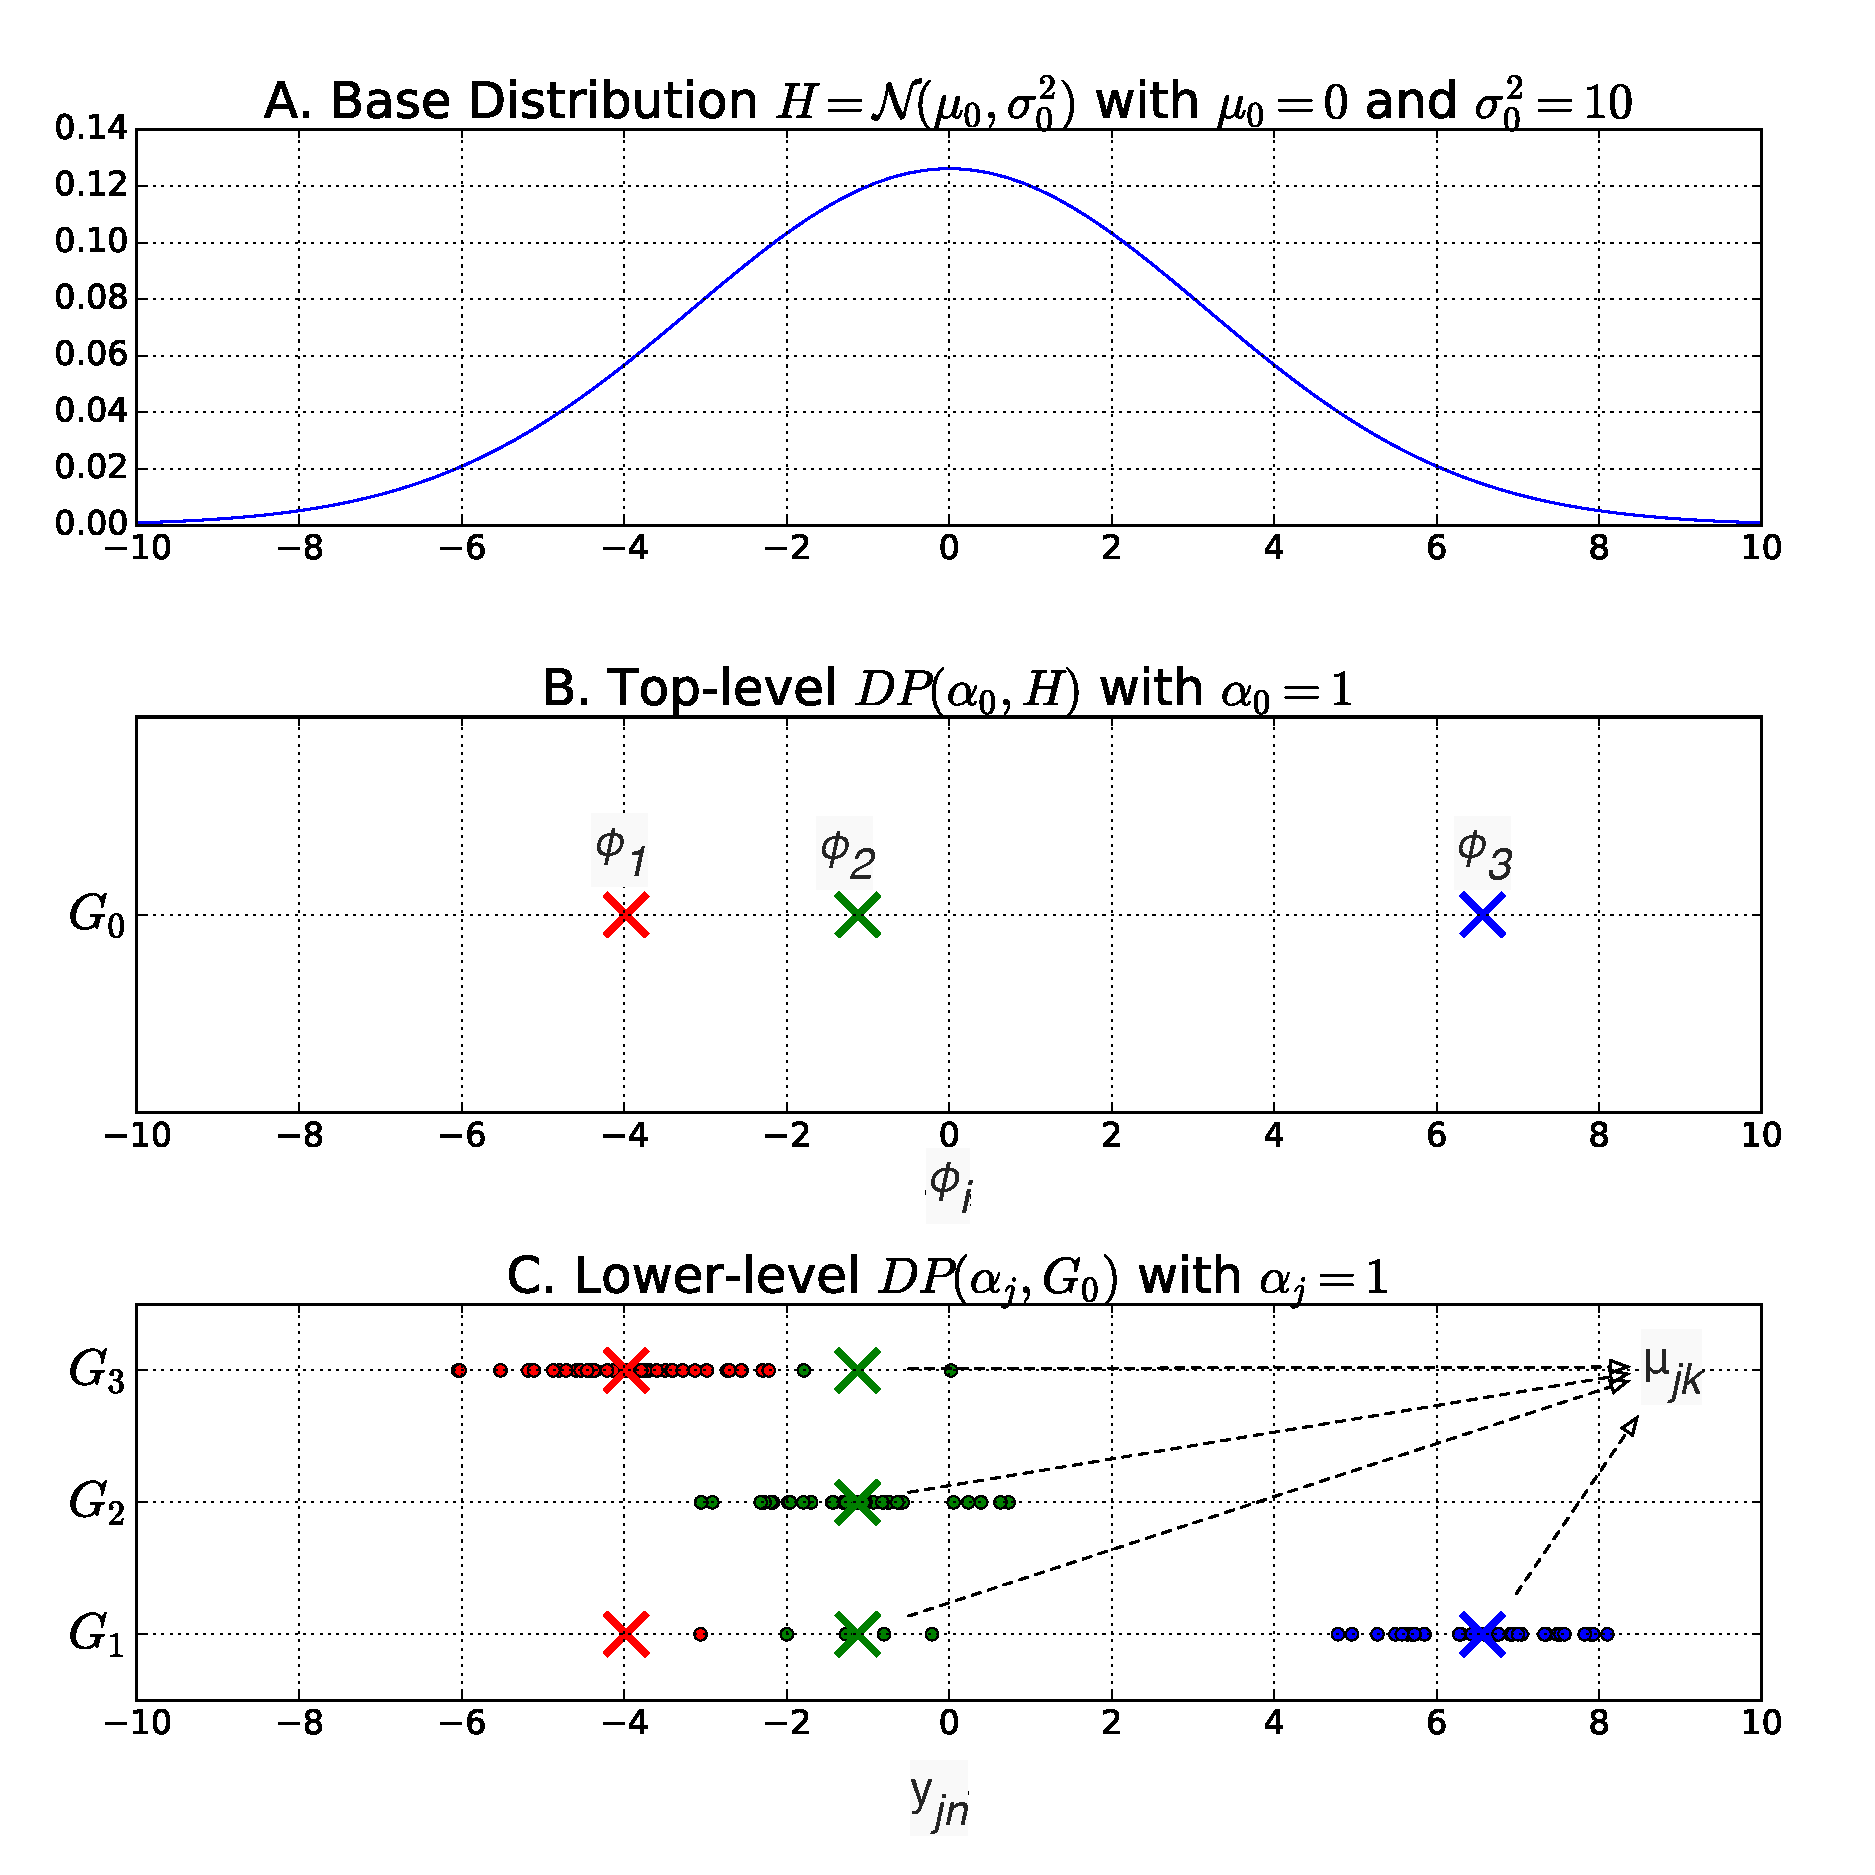
\includegraphics[width=0.6\textwidth]{03-machine-learning/figures/hdp_samples.pdf}
\par\end{centering}
\caption{\label{fig:g-from-hdp}An illustration of the generative process for the HDP mixture model defined in eq. (\ref{eq:background-infinite-mixture-hdp}). Similar to the DP mixture, we have a base distribution shown in \textbf{(A)}. Given $H$ and some concentration parameter $\alpha$, we generate a global distribution $G_0$. In \textbf{(B)}, we see that $G_0$ contains three unique discrete values. We then generate a file-specific distribution $G_j$ by sampling from a DP with $G_0$ as the base distribution. As a consequence, $G_j$ contains only discrete values copied from $G_0$. In \textbf{(C)}, the noisy observed values within each file is generated by sampling for $\mu_k$ from $G_j$, and sampling for $y_n$ conditioned on the $\mu_k$.}
\end{figure}

\subsection{Gibbs Sampling for a Hierarchical Dirichlet Process Mixture Model}

Inference for the HDP mixture model can also be performed via a Gibbs sampling scheme. In the following subsections, we describe the construction of a Gibbs sampler for the HDP mixture model in eq. (\ref{eq:background-infinite-mixture-hdp}). This follows from the \emph{posterior sampling in the Chinese restaurant franchise} approach in Section 5.1 of \cite{teh2005hierarchical}. In addition, we also describe in Chapter~\ref{c:hdp} the construction of a more elaborate Gibbs sampling scheme for the HDP-Align model.

As a preliminary to the Gibbs sampler, the following indices are defined: $j=1,...,J$ indexes over the files, $n=1,...,N$ indexes peaks in a $j$-th file (assume that all files have the same number of peaks), $k=1,...,K$ indexes the local clusters in a $j$-th file and $i=1,...,I$ indexes the shared global clusters across all files. Within a $j$-th file, the observed data is the RT values of peaks, denoted by $\boldsymbol{y}_j=\{y_{j1}, y_{j2}, ..., y_{jn}\}$. At any point in the sampler, the set of local cluster parameters (means) in the $j$-th file is denoted by $\{\mu_{j1}, \mu_{j2}, ..., \mu_{jk},\}$, while the set of global cluster parameters across all files is denoted by $\{\phi_1, \phi_2, ..., \phi_i\}$. Note that each local cluster parameter is a copy of a global cluster parameter in a particular file. When the global parameter is updated, all its local copies are updated too.

We also require keeping track of some count variables, namely $c_{jk}$ the number of peaks currently assigned to the $k$-th local cluster in the $j$-th file and $c_{i}$ the number of local clusters from all files currently assigned to the $i$-th global cluster. Note that both counts should exclude the object being sampled in the current iteration of the Gibbs sampler.

The conditional updates for the Gibbs sampler are given as follows:

\begin{enumerate}

\item \textbf{Assigning Peaks to Local Clusters}

Let the indicator variable $z_{jnk}=1$ denote the assignment of peak $n$ in file $j$ to an existing local cluster $k$ in the same file. Additionally, $z_{jnk^{*}}=1$ denotes the assignment of peak $n$ in file $j$ to a new local cluster $k^{*}$. For Gibbs sampling, we need to derive the conditional probability of $P(z_{jnk}=1)$ given the current peak RT value $y_{jn}$ and other model parameters. We denote this by $P(z_{jnk}=1 \vert y_{jn}, ...)$, where $...$ refers to other parameters being conditioned upon but not explicitly listed. Similar to the single-file collapsed Gibbs sampling in eq. (\ref{eq:background-infinite-mixture-model-sampling}), this conditional probability is given by:
\begin{dmath}
P(z_{jnk}=1 \vert y_{jn}, ...)\propto\begin{cases}
\begin{array}{c}
c_{jk}\cdot p(y_{jn} \vert z_{jnk}=1,...)\\
\alpha_{j}\cdot p(y_{jn} \vert z_{jnk^{*}}=1,...)
\end{array}\end{cases}\label{eq:background-hdp-conditional}
\end{dmath}

The conditional prior in eq. (\ref{eq:background-hdp-conditional}) is also known as the Chinese Restaurant Franchise (CRF), which can be seen as an extension of the CRP (described in Section~\ref{background-cgs-dpmixture}) that accommodates multiple files. In the CRF, a file now corresponds to a restaurant, each with an infinite number of tables. A new customer arrives at a restaurant and is assigned to an existing table with probability proportional to $c_{jk}$ (the number of other customers already sitting at the table $k$ in file $j$) or to a new table with probability proportional to $\alpha_j$ (the concentration parameter of the lower-level DP in file $j$). Across all restaurants, a global menu of dishes is maintained. The first customer who sits at a new table orders a dish from the global menu, which is shared by any subsequent customers who join that table. Existing dishes are served to the table with probability proportional to $c_i$ (the number of tables across the entire franchise already served the $i$-th dish), while a new dish is created with probability proportional to $\alpha_0$ (the concentration parameter of the top-level DP).

For the assignment of a data point $y_{jn}$ to a local cluster, a customer in the CRF analogy corresponds to a peak, a table is a local cluster parameter while a dish is a global cluster parameter. We consider the top and bottom terms of eq. (\ref{eq:background-hdp-conditional}) separately. The top term $p(y_{jn} \vert \boldsymbol{z}_{jnk}=1,...)$ is the probability of assigning the data point to an existing $k$-th local cluster in file $j$ having the cluster mean $\mu_{jk}$. This is proportional to $c_{jk}$ multiplied by the likelihood $\mathcal{N}(y_{jn} \vert \mu_{jk}, \sigma^2)$. The bottom term $p(y_{jn} \vert z_{jnk^{*}}=1,...)$ is the probability of assigning the data point to a new local cluster $k^{*}$. This is proportional to $\alpha_j$, multiplied by the likelihood of $y_{jn}$ under the new local cluster. To evaluate this likelihood, first we generate a new cluster mean $\mu_{jk^{*}}$ by sampling from the top-level Dirichlet Process $DP(\alpha_0, H)$. Let ${\phi_1, \phi_2, ... \phi_i}$ be the currently existing global cluster parameters shared across files. With probability proportional to $c_{i}$, an existing $\phi_{i}$ is instantiated as a new local cluster mean $\mu_{jk^{*}}$ in file $j$. Alternatively, with probability proportional to $\alpha_0$, a new $\phi_{i^{*}}$ is sampled from the base distribution $\mathcal{N}(\mu_0, \sigma_0^2)$ and instantiated as a new $\mu_{jk^{*}}$ in file $j$.

\item \textbf{Assigning Local Clusters to Global Clusters}

As the next step of the Gibbs sampler, we can also sample the assignment of a local cluster $k$ (and its entire member peaks) in file $j$ to a global cluster, allowing for multiple data points to be moved at the same time. This%at a may lead to an improved performance. % In theory, this may lead to an improved performance, however the probability of a successful reassignment of an entire local cluster to another existing global cluster is expected to be small since the prior \cite{teh2005hierarchical}

Let the indicator variable $v_{jki}=1$ denote the assignment of a local cluster $k$ in file $j$ to an existing global cluster $i$, and $v_{jki^*}=1$ denote the assignment of the local cluster to a new global cluster $i^*$. Furthermore, at any point in the sampler, let $\boldsymbol{x}_{jk}=\{x_{j1}, x_{j2}, ..., x_{jm}\}$ be the RT values of peaks currently assigned to the local cluster $k$ in file $j$, and there are $M_{jk}$ such peaks. 

Similar to eq. (\ref{eq:background-hdp-conditional}), the conditional prior for the assignment of a local cluster to a global cluster follows the CRP, resulting in:
\begin{dmath}
P(v_{jki}=1 \vert \boldsymbol{x}_{jk}, ...)\propto\begin{cases}
\begin{array}{c}
c_{i}\cdot p(\boldsymbol{x}_{jk} \vert v_{jki}=1,...)\\
\alpha_{0}\cdot p(\boldsymbol{x}_{jk} \vert v_{jki^{*}}=1,...)
\end{array}\end{cases}\label{eq:background-hdp-conditional-top-level}
\end{dmath}
In eq. (\ref{eq:background-hdp-conditional-top-level}), $p(\boldsymbol{x}_{jk} \vert v_{jki}=1,...)$ is given by the likelihood of the member peaks $\boldsymbol{x}_{jk}$ of local cluster $k$ in file $j$ to be placed under a global cluster $i$ with parameter $\phi_{i}$, therefore $p(\boldsymbol{x}_{jk} \vert v_{jki}=1,...) = \prod_{m=1}^{M_{jk}} \mathcal{N}(x_{jm} \vert \phi_{i}, \sigma^2)$ following our assumed independence assumption. Similarly, to evaluate $p(\boldsymbol{x}_{kj} \vert v_{jki^{*}}=1,...)$, first we sample for a new $\phi_{i^{*}}$ from the base distribution $\mathcal{N}(\mu_0, \sigma_0^2)$ and evaluate the data likelihood of $\boldsymbol{x}_{jk}$ under $\phi_{i^{*}}$. 

\item \textbf{Updating Other Parameters}

As the last step of our Gibbs sampler, we update each of global cluster parameter $\phi_i$ (and also its instantiated copies in each of the $j$-th file). For a particular $i$-th global cluster, this depends on the observations currently associated to it via any of the local clusters. We now denote by $\boldsymbol{x}_{i}$ the set of RT values of peaks currently assigned to the $i$-th global cluster from across all the files, and there are $M_i$ such peaks. The posterior density for $\phi_i$ is given by:
\begin{equation}
p(\phi_i \vert \boldsymbol{x}_i, \mu_0, ..) \propto \mathcal{N}(\phi_i \vert \mu_0, \sigma_0^2) \prod_{m=1}^{M_i} \mathcal{N}(x_i \vert \phi_i, \sigma^2)
\end{equation}
As in eq. (\ref{eq:background-tilde-mu-sigma}) for the single-file DP mixture case, this posterior can be simplified into another Gaussian $\mathcal{N}(\phi_i \vert \tilde{\mu}, \tilde{\sigma}^2)$ parameterised by:
\begin{equation}
\tilde{\mu} = \tilde{\sigma}^2 \bigg( \frac{\sum_{m=1}^{M_i} x_m}{\sigma^2} + \frac{\mu_0}{\sigma_0^2} \bigg), \enspace
\tilde{\sigma}^2 = \frac{1}{\frac{M}{\sigma^2} + \frac{1}{\sigma^2_0}} 
\label{eq:background-tilde-hdp-posterior}
\end{equation}
Appendix A in \cite{teh2005hierarchical} also describes how the DP concentration parameters for each $\alpha_j$ and also the $\alpha_0$ can be updated..

\end{enumerate}

This completes the Gibbs sampler for the HDP mixture model defined in eq. (\ref{eq:background-infinite-mixture-hdp}). We initialise the sampler by putting all peaks in the same file into one local cluster and assign all local clusters into one global cluster. The sampler then operates by repeating the three steps: re-sampling local cluster membership for all RT values following step (1) above, and re-sampling the local cluster to global cluster membership for all local clusters following step (2) above, and finally updating the parameters as in step (3). During the re-sampling steps, we keep track of which existing local clusters are empty in file $j$ via the count variables $\{c_{j1}, c_{j2}, ..., c_{jk}\}$. An empty table cannot have any new member assigned to it and can be deleted. Upon deleting a local cluster, we also update the global counter $c_{i}$ that tracks how many local clusters across all files are assigned to the $i$-th global cluster. A global cluster that is empty (not instantiated in any file) is also deleted. 

As the Gibbs sampling procedure above has shown (and also as can be observed from Figure~\ref{fig:g-from-hdp}), we see that within a file-specific $G_j$, each discrete value for $\mu_{jk}$ is copied exactly from the discrete values of $\phi_i$ from the global $G_0$. This may not be what we want. In particular, for our application, the top-level $G_0$ is the prior distribution over global compounds, which can be expected to correspond to metabolites (for metabolomics data) or peptide fragments (for proteomics data). The sample from a file-specific DP, denoted by $G_j$, is the prior distribution over the realisation of those compounds within a file. It is reasonable to expect the discrete values in $G_j$ to vary from $G_0$ with some random noise that represents the RT drift in the observed peaks. The addition of noise in this manner results in the `HDP with random effects' model \cite{kim2006hierarchical}. In Chapter~\ref{c:hdp}, we propose HDP-Align, a HDP mixture model that resembles \cite{kim2006hierarchical} but incorporates other LC-MS specific information, such as the m/z and RT values, to cluster peaks hierarchically across multiple files. Beyond clustering, the model is used to induce alignment (matching) of peaks from different files by placing peaks by placing them into the same RT and m/z clusters.

\section{Latent Dirichet Allocation\label{background-lda}}

We now turn our attention to an extension of the standard mixture model. In the standard mixture setting, a set of related data points that can be grouped together are said to be explained by a cluster (a probability distribution). For instance, a set of peaks are related through having close RT values. They can be grouped together under one cluster, and following the generative process, we assume that all observations in the same group are produced by a single probability distribution. In this section, we relaxes that assumption and introduces Latent Dirichlet Allocation (LDA) \cite{Blei2003}, another generative model that allows for related data points in the same group to be produced by a mixture of distributions instead.

The classical application of LDA lies for topic discovery for the text domain, although LDA-like models have been applied to continuous data \cite{rogers2005latent,weinshall2013lda,das2015gaussian}. In the text application, data points are the individual words, which can be grouped, forming a document. In a document, certain words tend to co-occur together --- for instance, `bayesian' and `probability' are two such words -- and ignoring word orders, we can represent this pattern of co-occurrences by a multinomial distribution the counts of words in a document. In the standard mixture model construction, we would have a document assigned to a cluster, and all words from the same document generated by sampling from the same multinomial distribution linked to the cluster. LDA relaxes that assumption by allowing for a document to contain words generated by a mixture of different \emph{topics}. A topic in this case still corresponds to a multinomial distribution over the entire vocabulary space.

We now describe the LDA model for text. Let $n=1,...,N$ indexes the unique words (vocabularies) and $d=1,...,D$ indexes the documents in our collection. Thus $w_{dn}$ refers to the $n$-th word in the $d$-th document. We also require the index $k=1,...,K$ over the topics, and let $z_{dn}$ to refer to the assignment of $w_{dn}$ to any of the $k$-th topic. The generative process for LDA is given as follows. For each $d$-th document, we sample a multinomial $\boldsymbol{\theta}_{d}$ over the $K$ topics. This document-to-topic distribution provides the mixture proportions of topics that explain the words in the document. Each document is also associated to a $\boldsymbol{z}_d$, the vector of assignment of its words to topics. Then for each word in the document, we sample $z_{dn}$, the assignment of the $n$-th word in the $d$-th document to a particular $k$-th topic. Given $z_{dn}=k$, we generate the actual word $w_{dn}$ by sampling from the $k$-th topic-to-word distribution $\boldsymbol{\phi}_{z_{dn}}$ that this word is assigned to through $z_{dn}=k$. A prior Dirichlet distribution parameterised by $\alpha$ is placed on the document-to-topic multinomials, and similarly, another prior Dirichlet parameterised by $\beta$ is placed on the topic-to-word multinomials. The generative model for LDA can be summarised as the following, and is illustrated in Figure~\ref{fig:background-lda}
\begin{equation}
\begin{aligned}
w_{dn} \vert \boldsymbol{\phi}_{z_{dn}} &\sim Multinomial(\boldsymbol{\phi}_{z_{dn}}) \\
z_{dn} \vert \boldsymbol{\theta}_{d}      &\sim Multinomial(\boldsymbol{\theta}_{d}) \\
\boldsymbol{\theta}_{d} \vert \boldsymbol{\alpha}                &\sim Dir(\boldsymbol{\alpha}) \\ 
\boldsymbol{\phi}_{k} \vert \boldsymbol{\beta}                     &\sim Dir(\boldsymbol{\beta})
\end{aligned}
\label{eq:background-lda-model}
\end{equation}

\begin{figure}[tbh!]
\noindent \begin{centering}
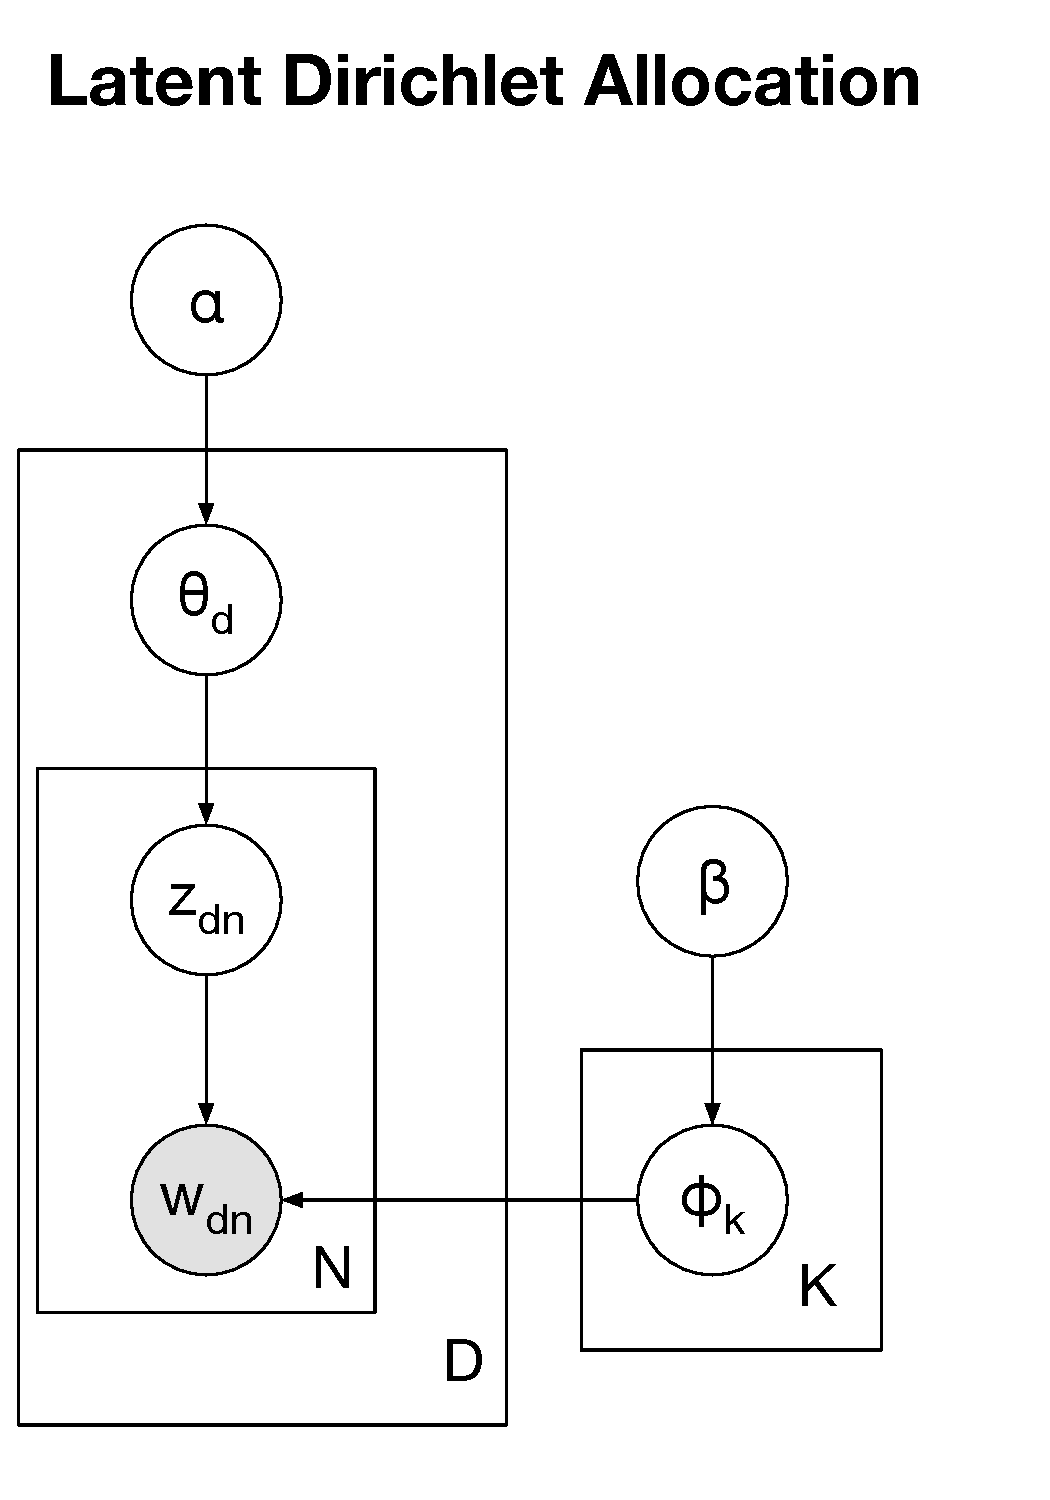
\includegraphics[width=0.5\textwidth]{03-machine-learning/figures/lda.pdf}
\par\end{centering}
\caption{\label{fig:background-lda}Graphical model of the Latent Dirichlet Allocation model. Circles denotes random variables, while the shaded node denotes the observed word value.}
\end{figure}

To state the joint distribution of the model, we need to define more notations. Let $\boldsymbol{W}=\{\boldsymbol{w}_1, \boldsymbol{w}_2, ..., \boldsymbol{w}_d\}$ denote the entire collection of documents and $\boldsymbol{Z}$ denotes the entire set of assignment variables for all documents, $\boldsymbol{Z} = \{\boldsymbol{z}_1, \boldsymbol{z}_2, ..., \boldsymbol{z}_d\}$. We put the multinomial parameter sets for all the document-to-topic distributions into $\boldsymbol{\Theta}=\{\boldsymbol{\theta}_{1}, \boldsymbol{\theta}_{2}, ..., \boldsymbol{\theta}_{d}\}$. Similarly, the multinomial parameter sets for all topic-to-word distributions are put into $\boldsymbol{\Phi}=\{\boldsymbol{\phi}_1, \boldsymbol{\phi}_2, ..., \boldsymbol{\phi}_k\}$. Then the joint probability distribution is given by:
\begin{equation}
\begin{aligned}
p(\boldsymbol{W}, \boldsymbol{Z}, \boldsymbol{\Theta}, \boldsymbol{\Phi} \vert \boldsymbol{\alpha}, \boldsymbol{\beta}) &= p(\boldsymbol{\Phi} \vert \boldsymbol{\beta}) \cdot p(\boldsymbol{\Theta} \vert \boldsymbol{\alpha}) \cdot p(\boldsymbol{Z} \vert \boldsymbol{\Theta}) \cdot  p(\boldsymbol{W} \vert \boldsymbol{\Phi}, \boldsymbol{Z}) \\
                                                                                                                                                                                          &= \prod_{k=1}^{K} p(\boldsymbol{\phi}_k \vert \boldsymbol{\beta}) \cdot \prod_{d=1}^{D} p(\boldsymbol{\theta}_d \vert \boldsymbol{\alpha}) \cdot \prod_{d=1}^{D} \prod_{n=1}^{N} p(z_{dn} \vert \boldsymbol{\theta}_d) \cdot \prod_{d=1}^{D} \prod_{n=1}^{N} p(w_{dn} \vert \boldsymbol{\phi}_{z_{dn}})
\end{aligned}
\label{eq:background-lda-full-joint}
\end{equation}

\subsection{Collapsed Gibbs Sampling for Latent Dirichlet Allocation}

Similar to the mixture model case, inference in LDA can be performed via a collapsed Gibbs sampling scheme. In particular, we are interested in the conditional probability of $P({z}_{dn}=k \vert \boldsymbol{Z}^{-}, \boldsymbol{W}, \boldsymbol{\alpha}, \boldsymbol{\beta})$, the assignment of word $n$ in document $d$ to topic $k$ given other assignments and model hyperparameters. This is proportional to the joint distribution given in eq. (\ref{eq:background-lda-full-joint}). For collapsed Gibbs sampling in LDA, we also aim to integrate out the document-to-topic distributions $\boldsymbol{\Theta}$ and the topic-to-word distributions $\boldsymbol{\Phi}$ from the joint distribution in eq. (\ref{eq:background-lda-full-joint}). This results in: 
\begin{equation}
\begin{aligned}
P({z}_{dn}=k \vert \boldsymbol{Z}^{-}, \boldsymbol{W}, \boldsymbol{\alpha}, \boldsymbol{\beta}) &\propto \int_{\boldsymbol{\Theta}} \int_{\boldsymbol{\Phi}} p(\boldsymbol{W}, \boldsymbol{Z}, \boldsymbol{\Theta}, \boldsymbol{\Phi} \vert \boldsymbol{\alpha}, \boldsymbol{\beta}) \enspace d\boldsymbol{\Theta} \enspace d\boldsymbol{\Phi} \\
                                                                                                                                                    &\propto \int_{\boldsymbol{\Theta}} \int_{\boldsymbol{\Phi}} p(\boldsymbol{\Phi} \vert \boldsymbol{\beta}) \cdot p(\boldsymbol{\Theta} \vert \boldsymbol{\alpha}) \cdot p(\boldsymbol{Z} \vert \boldsymbol{\Theta}) \cdot  p(\boldsymbol{W} \vert \boldsymbol{\Phi}, \boldsymbol{Z}) \enspace d\boldsymbol{\Theta} \enspace d\boldsymbol{\Phi} \\
                                                                                                                                                    &\propto \Bigg[ \int_{\boldsymbol{\Theta}}  p(\boldsymbol{Z} \vert \boldsymbol{\Theta}) \cdot p(\boldsymbol{\Theta} \vert \boldsymbol{\alpha}) \enspace d\boldsymbol{\Theta} \Bigg] \Bigg[\int_{\boldsymbol{\Phi}} p(\boldsymbol{W} \vert \boldsymbol{\Phi}, \boldsymbol{Z}) \cdot p(\boldsymbol{\Phi} \vert \boldsymbol{\beta}) \enspace d\boldsymbol{\Phi} \Bigg] \\ 
\label{eq:lda-gibbs}
\end{aligned}
\end{equation}

The right hand side of eq. (\ref{eq:lda-gibbs}) can be separated into two parts: the prior term involving $\boldsymbol{Z}$, $\boldsymbol{\Theta}$ and $\boldsymbol{\alpha}$ and the data likelihood term involving $\boldsymbol{W}$, $\boldsymbol{\Phi}$ and $\boldsymbol{\beta}$. We denote the prior term by $p({z}_{dn}=k \vert ...)$ and the likelihood term by $p({w}_{dn} \vert {z}_{dn}=k, ...)$, where $...$ denotes any other parameters being conditioned upon but not explicitly listed. A derivation for eq. (\ref{eq:lda-gibbs}) can be found in \cite{carpenter2010integrating}, but here we briefly summarise the result.

For the prior term $p({z}_{dn}=k \vert ...)$, marginalising over all $\boldsymbol{\theta}_{d}$ parameters produces:
\begin{equation}
\begin{aligned}
P({z}_{dn}=k \vert ...) &= \int_{\boldsymbol{\Theta}}  p(\boldsymbol{Z} \vert \boldsymbol{\Theta}) \cdot p(\boldsymbol{\Theta} \vert \boldsymbol{\alpha}) \enspace d\boldsymbol{\Theta} \\
                                  &= \prod_{d=1}^{D} \int_{\boldsymbol{\theta}_d} \Bigg[ p(\boldsymbol{z}_{d} \vert \boldsymbol{\theta}_d) \cdot p(\boldsymbol{\theta}_d \vert \boldsymbol{\alpha}) \Bigg] d\boldsymbol{\theta}_d \\
\end{aligned}                                  
\label{eq:lda-gibbs-prior}
\end{equation}
After integrating the Dirichlet-Multinomial distribution from $p(\boldsymbol{z}_{d} \vert \boldsymbol{\theta}_d) \cdot p(\boldsymbol{\theta}_d \vert \boldsymbol{\alpha})$ in eq. (\ref{eq:lda-gibbs-prior}) and simplifying the resulting expression that contains gamma functions, it can be shown in \cite{carpenter2010integrating} that eq. (\ref{eq:lda-gibbs-prior}) reduces to this simple expression:
\begin{equation}
P({z}_{dn}=k \vert ...) \propto  c_{dk} + {\alpha}_k
\label{eq:lda-gibbs-prior-simple}
\end{equation}
with $c_{dk}$ the number of words from document $n$ currently assigned to topic $k$, excluding the current word being sampled. Similarly for the likelihood term of $P({w}_{dn} \vert {z}_{dn}=k, ...)$, marginalising over all $\boldsymbol{\phi}_k$ parameters produces:
\begin{equation}
\begin{aligned}
P({w}_{dn} \vert {z}_{dn}=k, ...) &= \int_{\boldsymbol{\Phi}} p(\boldsymbol{W} \vert \boldsymbol{\Phi}, \boldsymbol{Z}) \cdot p(\boldsymbol{\Phi} \vert \boldsymbol{\beta}) \enspace d\boldsymbol{\Phi} \\
                                                 &= \prod_{k=1}^{K} \int_{\boldsymbol{\phi}_k} \Bigg[ p(\boldsymbol{\phi}_k \vert \boldsymbol{\beta}) \cdot \prod_{d=1}^{D} \prod_{n=1}^{N} p(w_{dn} \vert \boldsymbol{\phi}_{z_{dn}}) \Bigg]\enspace d\boldsymbol{\phi}_k
\end{aligned}
\label{eq:lda-gibbs-likelihood}
\end{equation}
and it can be shown that eq. (\ref{eq:lda-gibbs-likelihood}) reduces to:
\begin{equation}
P({w}_{dn} \vert {z}_{dn}=k, ...) \propto \frac{c_{kn} + {\beta}_n}{\sum_{n} c_{kn} + {\beta}_n}
\label{eq:lda-gibbs-likelihood-simple}
\end{equation}
where $c_{kn}$ is the total number of the $n$-th word currently assigned to topic $k$, excluding the current word being sampled.  

Putting the prior and likelihood terms together, the following conditional distribution is obtained for the assignment of word $n$ in document $d$ to topic $k$:
\begin{equation}
P({z}_{dn}=k \vert \boldsymbol{Z}^{-}, \boldsymbol{W}, \boldsymbol{\alpha}, \boldsymbol{\beta}) \propto (c_{dk} + {\alpha}_k) \cdot \frac{ c_{kn} + {\beta}_n}{\sum_{n} c_{kn} + {\beta}_n}
\label{eq:lda-gibbs-combined}
\end{equation}

For each sample, we can also update the multinomial parameter sets $\boldsymbol{\Theta}=\{\boldsymbol{\theta}_{1}, \boldsymbol{\theta}_{2}, ..., \boldsymbol{\theta}_{d}\}$ for all documents and $\boldsymbol{\Phi}_k=\{\boldsymbol{\phi}_1, \boldsymbol{\phi}_2, ..., \boldsymbol{\phi}_k\}$ for all topics. Consider one $\boldsymbol{\theta}_{d}$, the multinomial parameter of the $d$-th document-to-topic distribution. This multinomial distribution has a prior Dirichlet distribution parameterised by $\alpha$ and the observed counts $c_{dk}$ of words from document $d$ to topic $k$. Applying Bayes rule, we obtain the updated posterior which takes the form of a Dirichlet-multinomial distribution parameterised by $Dir(c_{d1}+{\alpha}_1, c_{d2}+{\alpha}_2, ...,c_{dk}+{\alpha}_k)$. The same applies to $\boldsymbol{\phi}_{k}$, the multinomial parameter of the $k$-th topic-to-word distribution.

Using the expectation of the Dirichlet distribution, we obtain the updated value for $\theta_{dk}$ (the $k$-th entry in ${\boldsymbol{\theta}_{d}}$) and also ${\phi}_{kn}$ (the $n$-th entry in $\boldsymbol{\phi}_{k}$) as:
\begin{align}
{\theta}_{dk} = \frac{c_{dk}+{\alpha}_k}{\sum_{k} c_{dk}+{\alpha}_k}, \enspace {\phi}_{kn} = \frac{c_{kn}+{\beta}_n}{\sum_{n} c_{kn}+{\beta}_n}
\label{eq:background-lda-updated-theta-phi}
\end{align}
where $c_{dk}$ is the count of words from document $d$ assigned to topic $k$ and $c_{kn}$ is the count of the $n$-th words assigned to topic $k$. 

The collapsed Gibbs sampling for LDA then proceeds as follows: given $K$ topics, we initialise the sampler by randomly assigning words to topics and setting the count variables for $c_{dk}$ used in eq. (\ref{eq:lda-gibbs-prior-simple}) and for $c_{kn}$ used in eq. (\ref{eq:lda-gibbs-likelihood-simple}). We then iterate over the words in all documents, removing any information about it from the counts and computing the conditional probability of $P({z}_{dn}=k \vert {w}_{dn}, ...)$ using eq. (\ref{eq:lda-gibbs}). The word is assigned to the $k$-th topic, so we update the indicator variable ${z}_{dn}$ and other relevant count variables to reflect this assignment. We also obtain the updated multinomial parameters for $\boldsymbol{\theta}_d$ and $\boldsymbol{\phi}_k$ using eq. (\ref{eq:background-lda-updated-theta-phi}).

\section{Conclusion}

In this chapter, we have described the principle of mixture model clustering, with a particular example of its application to the generative modelling peak data by their retention time values. The mixture model starts by being a finite model, where the number of cluster is specified. With a Dirichlet Process prior, the mixture model is extended to an infinite model where the number of clusters grow with the data. Next, a hierarchical prior in form of the hierarchical Dirichlet Process is also introduced to let us deal with shared clustering across multiple input files. Finally, Latent Dirichlet Allocation is introduced to let us model ad-mixture data, where related items in a group is explained by a distribution of mixture. These models serve as the building blocks in the remaining parts of this thesis. In the coming Chapter~\ref{c:matching}, we explore the idea of using the information from peak grouping to improve the direct-matching alignment step that follows. In Chapter~\ref{c:precursor-clustering}, a mixture model is proposed to group ionisation product peaks by the set of user-defined chemical transformations. This grouping is again used to improve the alignment step. In Chapter~\ref{c:hdp}, a model based on the hierarchical Dirichle Process mixture is proposed to perform the grouping of ionisation product peaks across multiple runs, constructing alignment as a natural output and allowing for matching uncertainties of aligned peaksets to be returned to the user. Finally, in Chapter~\ref{c:lda}, an application of topic modelling is proposed to decompose fragmentation spectra into a set of co-occuring fragment peaks, allowing for better hypothesis generations in the identification of metabolites present in the sample. Common to all the chapters are the idea that many peaks that exist in LC-MS data are not independent, but instead share chemically meaningful relationship and can be grouped. These groupings can be explained by some underying latent variables that potentially correspond to peptides or metabolites, and this information can be used to improve other steps in the LC-MS data pre-processing pipeline.